% !TEX program = pdflatex
\documentclass[letterpaper,12pt]{article}
\usepackage[spanish,mexico]{babel}
\usepackage[T1]{fontenc}
\usepackage{lmodern}
\usepackage{amsmath,amssymb}
\usepackage{graphicx,float,subcaption,xcolor,array,booktabs,tabularx,ragged2e}
\usepackage{tikz}
\usetikzlibrary{arrows.meta,positioning,shapes.geometric,calc}
\usepackage{listings}
\usepackage[left=25mm,right=25mm,top=35mm,bottom=30mm,headheight=15pt]{geometry}
\usepackage{parskip,fancyhdr}
\usepackage{hyperref}

\graphicspath{{img/}{portada_img/}}
\newcommand{\materia}{Laboratorio de Organización y Arquitectura de Computadoras}
\pagestyle{fancy}
\fancyhf{}
\fancyhead[R]{\textsc{\materia}}
\fancyfoot[C]{\thepage}
\renewcommand{\headrulewidth}{0.8pt}
\hypersetup{colorlinks=true,linkcolor=blue,urlcolor=cyan}

\definecolor{codebg}{rgb}{0.96,0.96,0.96}
\definecolor{keyword}{rgb}{0.0,0.2,0.6}
\definecolor{comment}{rgb}{0.25,0.5,0.35}
\definecolor{codegray}{rgb}{0.5,0.5,0.5}
\lstdefinestyle{estiloVHDL}{
  language=VHDL,basicstyle=\ttfamily\scriptsize,
  backgroundcolor=\color{codebg},commentstyle=\color{comment}\itshape,
  keywordstyle=\color{keyword}\bfseries,numbers=left,
  numberstyle=\tiny\color{codegray},frame=single,breaklines=true,
  literate={á}{{\'a}}1 {é}{{\'e}}1 {í}{{\'i}}1 {ó}{{\'o}}1 {ú}{{\'u}}1 {ñ}{{\~n}}1,
  keepspaces=true,showstringspaces=false,tabsize=4,
  morekeywords={library,use,all,entity,is,port,in,out,architecture,of,begin,end,signal,constant,process,if,then,else,elsif,case,when,others,std_logic,std_logic_vector}
}

\begin{document}
\thispagestyle{empty} % Sin encabezado ni pie en la portada

% --- ENCABEZADO DE PORTADA (TABLA DE 3 COLUMNAS) ---
\begin{center}
    % La tabla usa 'm' para centrar verticalmente las imágenes y el texto
    \begin{tabular}{m{0.15\textwidth} m{0.60\textwidth} m{0.15\textwidth}}
        % Logo Izquierdo (UNAM)
        
\includegraphics[width=2cm]{portada_img/escudounam_negro.jpg} & 
        
        % Título Central
        \centering\Huge\textbf{Universidad Nacional Autónoma de México} &
        
        % Logo Derecho (Facultad)
        \raggedleft
\includegraphics[width=2cm]{portada_img/escudofi_negro.jpg}
    \end{tabular}
\end{center}

\vspace{0.3cm}

% --- INFORMACIÓN DEL REPORTE ---
\begin{center}
    {\LARGE \textbf{Facultad de Ingeniería}}\\[1cm]

    {\LARGE \textbf{Laboratorio de Arquitectura y Organización de Computadoras}} \\[1cm]

	{\LARGE Grupo: 07 - Semestre: 2027-1} \\[1cm]
    
    {\LARGE \textbf{Reporte Practica 5}}\\[0.5cm]
    {\LARGE {Construción de Máquinas de estados Usando Memorias Direccionamiento Implícito}}\\[1cm]

    {\Large \textbf{Fecha de Entrega}}\\[0.2cm]
    {\Large 10 de Octubre del 2026} \\[1cm]

    {\LARGE \textbf{Profesor}}\\[0.2cm]
    {\Large Ing. Julio Cesar Cruz Estrada}\\[1cm]
    
    {\LARGE \textbf{Integrantes:}}\\[0.2cm]
    {\Large Espinoza Matamoros Percival Ulises}\\[0.5cm]
    {\Large Montiel Juárez Oscar Iván}\\[0.5cm]
    {\Large Veraza García Amy Valentina}\\[0.5cm]

\end{center}
\newpage

\section{Objetivo}

Familiarizar al alumno en el conocimiento de construcción de máquinas de estados usando direccionamiento de memorias con el método de direccionamiento implícito.

\section{Desarrollo}

El direccionamiento implícito aprovecha el orden consecutivo de los estados. Para cada estado presente $N$, una de las dos transiciones posibles no se almacena en la memoria, sino que se obtiene mediante un incrementador como $N+1$. La otra transición, denominada liga $P$, sí se guarda en la palabra de control. Para utilizar este método, la asignación binaria debe cumplir la regla $N$, $N+1$, $P$. Cuando la carta ASM original no la cumple, es necesario reasignar los códigos de estado.

La palabra almacenada también contiene el código de la entrada que se debe probar, el bit $VF$ y dos campos de salida. El bit $VF$ indica con qué valor de la entrada seleccionada se debe utilizar la liga explícita. Si el resultado de la prueba coincide con $VF$, el contador carga $P$, en caso contrario, avanza a $N+1$. De esta manera, sólo se almacena una liga de tres bits en lugar de dos.

\subsection{Carta ASM y asignación binaria}

La carta ASM utilizada tiene seis estados, tres entradas de decisión y cuatro salidas. Las entradas $A$, $B$ y $C$ se codificaron como \texttt{00}, \texttt{01} y \texttt{10}; el código \texttt{11} se reservó para $QAUX$. En la implementación, $QAUX$ se conecta a cero y permite representar estados sin prueba externa.

\begin{figure}[H]
\centering
\begin{tikzpicture}[
  flow/.style={-{Stealth[length=2.4mm,width=1.6mm]}, line width=0.8pt, rounded corners=2pt},
  state/.style={draw, rectangle, minimum width=2.4cm, minimum height=0.85cm, align=center},
  decision/.style={draw, diamond, aspect=1.3, minimum width=1.1cm, minimum height=0.85cm, inner sep=1pt},
  condout/.style={draw, ellipse, minimum width=1.7cm, minimum height=0.75cm, align=center},
  every node/.style={font=\small},
  elbl/.style={font=\small\bfseries\color{red}} % Estilo para los identificadores de estado
]

  % --- ESTADOS Y DECISIONES ---
  % Estado inicial E0 y decisión A
  \node[state, label={[elbl]above:$E_0$}] (e0) at (0, 0) {$S_3 S_2 \overline{S_1}\,\overline{S_0}$};
  \node[decision] (a) at (0, -1.6) {$A$};

  % Rama izquierda: E1, B, condout S1, E2, E3
  \node[state, label={[elbl]above right:$E_1$}] (e1) at (-3.2, -3.1) {$\overline{S_3}\,\overline{S_0}$};
  \node[decision] (b) at (-3.2, -4.6) {$B$};
  \node[condout] (bsalida) at (-1.4, -5.8) {$\overline{S_1}$};
  \node[state, label={[elbl]above left:$E_2$}] (e2) at (-1.4, -7.2) {\phantom{$S_0$}}; % Caja vacía con altura uniforme
  \node[state, label={[elbl]above left:$E_3$}] (e3) at (-4.8, -7.2) {$S_2$};

  % Rama derecha: E4, C, E5
  \node[state, label={[elbl]above right:$E_4$}] (e4) at (3.2, -3.1) {$S_2 \overline{S_1}$};
  \node[decision] (c) at (3.2, -4.6) {$C$};
  \node[state, label={[elbl]above right:$E_5$}] (e5) at (3.2, -6.3) {$\overline{S_0}$};

  % --- CONEXIONES Y FLUJOS ---
  % Desde E0 hasta A
  \draw[flow] (e0) -- (a);

  % Decisión A (1 -> E1, 0 -> E4)
  \draw[flow] (a.west) -| node[above, pos=0.25] {$1$} (e1.north);
  \draw[flow] (a.east) -| node[above, pos=0.25] {$0$} (e4.north);

  % Rama izquierda
  \draw[flow] (e1) -- (b);
  \draw[flow] (b.west) -| node[above, pos=0.25] {$0$} (e3.north);
  \draw[flow] (b.east) -| node[above, pos=0.25] {$1$} (bsalida.north);
  \draw[flow] (bsalida) -- (e2.north);

  % Conexión E2 -> E3
  \draw[flow] (e2.west) -- (e3.east);

  % Rama derecha
  \draw[flow] (e4) -- (c);
  \draw[flow] (c.south) -- node[right] {$0$} (e5.north);

  % Transición E5 -> E2
  \draw[flow] (e5.south) |- ([yshift=-4mm]e2.south) -| (e2.south);

  % Retorno E4 (C = 1) -> E0
  \draw[flow] (c.east) -- node[above, pos=0.2] {$1$} (5.2, -4.6)
    |- ([xshift=8mm, yshift=7mm]e0.north)
    -- ([xshift=8mm]e0.north);

  % Retorno E3 -> E0
  \draw[flow] (e3.west) -- (-6.3, -7.2)
    |- ([xshift=-8mm, yshift=7mm]e0.north)
    -- ([xshift=-8mm]e0.north);

\end{tikzpicture}
\caption{Carta ASM empleada utilizada para la práctica 5.}
\label{fig:carta-asm}
\end{figure}


La asignación binaria seleccionada es:
\[
\begin{array}{c|cccccc}
\text{Estado} & E_0 & E_1 & E_2 & E_3 & E_4 & E_5\\ \hline
Q_2Q_1Q_0 & 000 & 001 & 010 & 011 & 100 & 101
\end{array}
\qquad
\begin{array}{c|cccc}
\text{Entrada} & A & B & C & QAUX\\ \hline
K_1K_0 & 00 & 01 & 10 & 11
\end{array}
\]

Con esta codificación se obtienen las siguientes transiciones:
\[
\begin{aligned}
E_0 &: A=0\rightarrow E_4,\quad A=1\rightarrow E_1,\\
E_1 &: B=0\rightarrow E_3,\quad B=1\rightarrow E_2,\\
E_2 &: E_3,\qquad
E_3 : E_0,\\
E_4 &: C=0\rightarrow E_5,\quad C=1\rightarrow E_0,\\
E_5 &: E_2.
\end{aligned}
\]
Las transiciones $E_0\rightarrow E_1$, $E_1\rightarrow E_2$, $E_2\rightarrow E_3$ y $E_4\rightarrow E_5$ corresponden a $N+1$ y, por tanto, pueden generarse sin guardar una segunda liga.

\subsection{Dimensionamiento de la memoria}

Se requieren tres bits para representar los seis estados, por lo que la memoria dispone de $2^3=8$ direcciones. La palabra de control se organiza de la siguiente forma:
\[
\underbrace{K_1\,K_0}_{\text{prueba}}
\;\underbrace{VF}_{\text{valor de liga}}
\;\underbrace{L_2\,L_1\,L_0}_{\text{liga }P}
\;\underbrace{SF_3\,SF_2\,SF_1\,SF_0}_{\text{salida falsa}}
\;\underbrace{SV_3\,SV_2\,SV_1\,SV_0}_{\text{salida verdadera}}.
\]
Por lo tanto, el número de bits por palabra es
\[
m=2+1+3+4+4=14\ \text{bits},
\]
y el tamaño de la memoria es
\[
2^n\times m=2^3\times14=8\times14=112\ \text{bits}.
\]
Aunque sólo se emplean seis estados, se programaron también las direcciones \texttt{110} y \texttt{111} con valores seguros para regresar a \texttt{000}.

\subsection{Tabla de direccionamiento y contenido de la memoria}

La Tabla[\ref{tab:memoria}] muestra el programa grabado en la ROM. Donde $K_1K_0$ selecciona la entrada, $VF$ determina cuándo se carga la liga explícita y $L_2L_1L_0$ contiene $P$. Los campos $SF$ y $SV$ se seleccionan cuando la entrada evaluada vale \texttt{0} o \texttt{1}.

\begin{table}[H]
\centering
\scriptsize
\caption{Tabla de direccionamiento implícito y contenido de la ROM.}
\label{tab:memoria}
\begin{tabular}{c c c c c c}
\toprule
Estado & $Q_2Q_1Q_0$ & $K_1K_0$ & $VF$ & Liga $P$ & $SF/SV$\\
\midrule
$E_0$ & 000 & 00 & 0 & 100 & 1100/1100\\
$E_1$ & 001 & 01 & 0 & 011 & 1010/1000\\
$E_2$ & 010 & 11 & 1 & 000 & 0011/0011\\
$E_3$ & 011 & 11 & 0 & 000 & 0111/0111\\
$E_4$ & 100 & 10 & 1 & 000 & 0101/0101\\
$E_5$ & 101 & 11 & 0 & 010 & 0010/0010\\
Recuperación & 110 & 11 & 0 & 000 & 0011/0011\\
Recuperación & 111 & 11 & 0 & 000 & 0011/0011\\
\bottomrule
\end{tabular}
\end{table}

Por ejemplo, en $E_0$ la ROM entrega \texttt{00 0 100 1100 1100}. El código \texttt{00} selecciona $A$. Si $A=0$, su valor coincide con $VF=0$ y se carga la liga explícita \texttt{100} si $A=1$, no coincide con $VF$ y el incrementador produce \texttt{001}. En ambos casos la salida es \texttt{1100}.

\subsection{Arquitectura del sistema}

El registro entrega el estado presente, que funciona como dirección de la ROM y como entrada del incrementador. La ROM genera los campos de prueba, $VF$, liga y salidas. El multiplexor de prueba selecciona $A$, $B$, $C$ o $QAUX$ y produce $Qsel$. Después, una compuerta XNOR compara $Qsel$ con $VF$ para generar la señal de carga:
\[
\texttt{carga}=\overline{Qsel\oplus VF}.
\]
Cuando \texttt{carga=1}, el multiplexor de control selecciona la liga $P$, cuando \texttt{carga=0}, selecciona $N+1$. En paralelo, \texttt{mux\_salida} escoge $SF$ o $SV$ directamente con $Qsel$.

\begin{figure}[H]
\centering
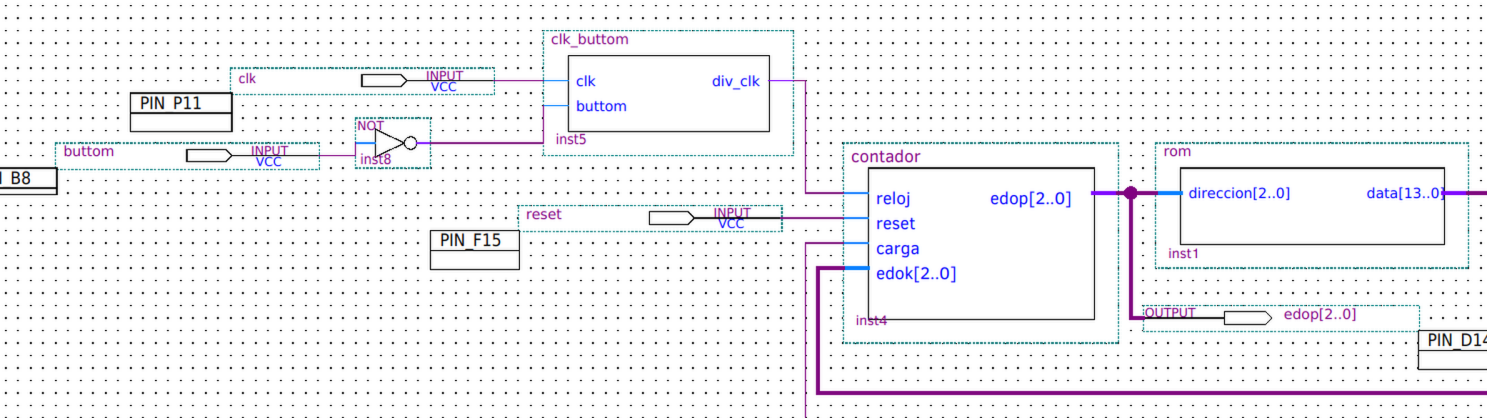
\includegraphics[width=\linewidth]{diagramas_bloques_1.png}
\caption{Conexión del reloj y del bloque contador dentro del sistema.}
\label{fig:bloques-1}
\end{figure}

La Figura[\ref{fig:contador-interno}] muestra la estructura interna del contador con carga. La salida \texttt{edop} del registro se realimenta hacia el incrementador, que produce \texttt{edouno=edop+1}. El multiplexor \texttt{mux\_control} recibe ese valor y la liga \texttt{edok} proveniente de la ROM. La señal \texttt{carga} decide cuál de los dos valores se aplica a \texttt{edos}, finalmente, el registro captura \texttt{edos} en el siguiente flanco ascendente de \texttt{reloj}. La entrada \texttt{reset} permite forzar el estado inicial \texttt{000}.

\begin{figure}[H]
\centering
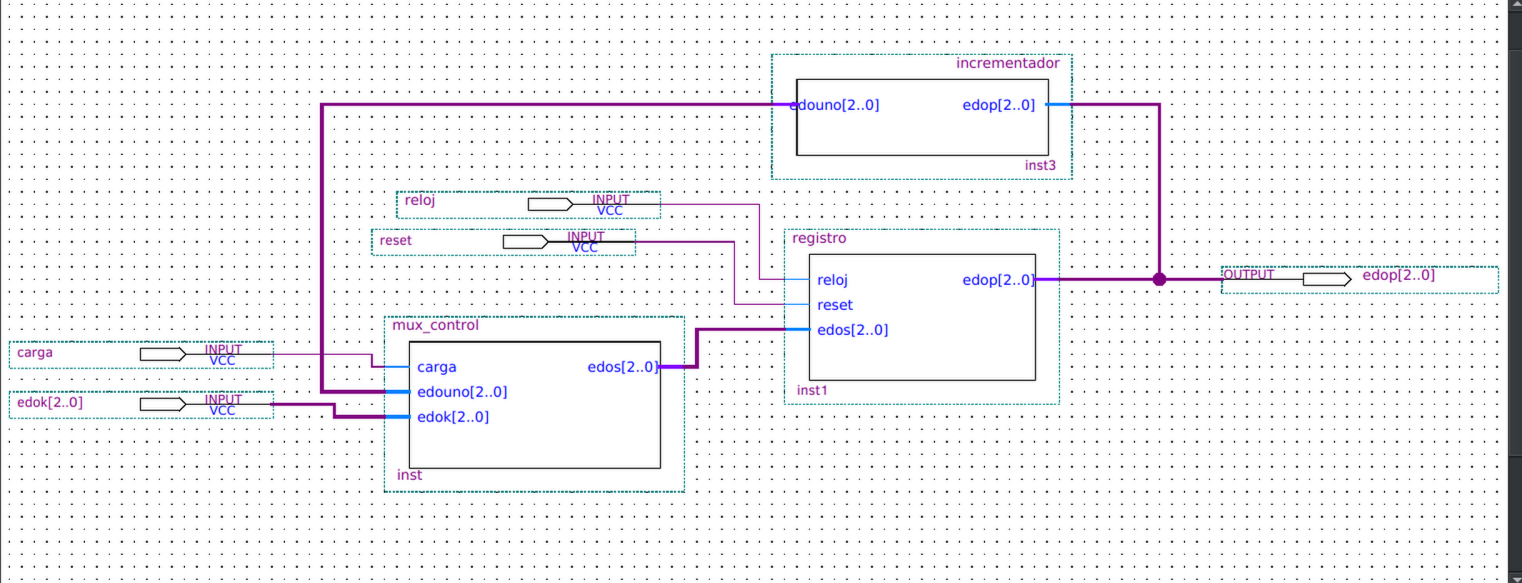
\includegraphics[width=\linewidth]{diagramas_bloques_4_contador.png}
\caption{Diagrama interno del contador con carga: multiplexor, registro e incrementador.}
\label{fig:contador-interno}
\end{figure}

\begin{figure}[H]
\centering
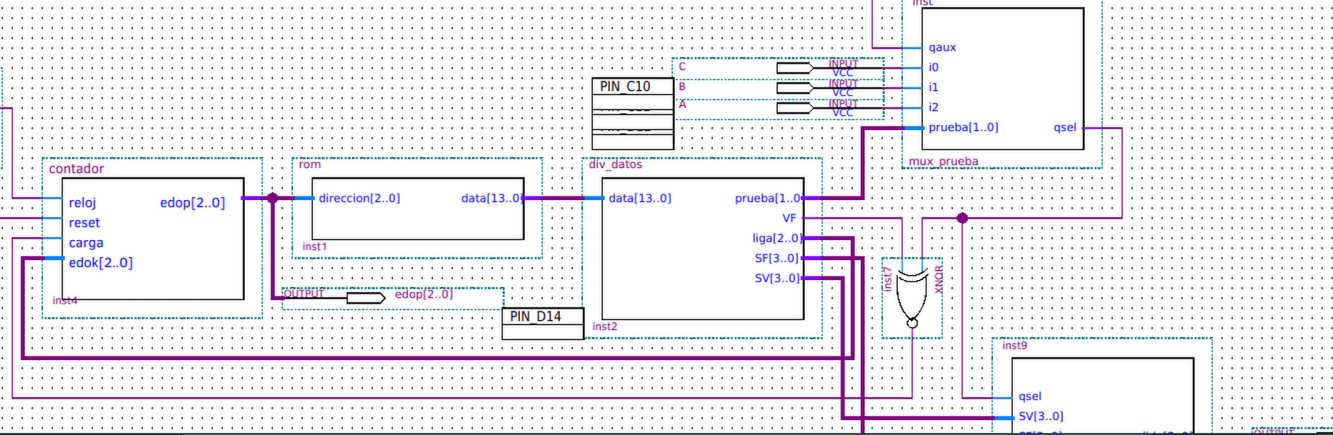
\includegraphics[width=\linewidth]{diagramas_bloques_2.png}
\caption{Conexión del contador, la ROM y la separación de la palabra de control.}
\label{fig:bloques-2}
\end{figure}

\begin{figure}[H]
\centering
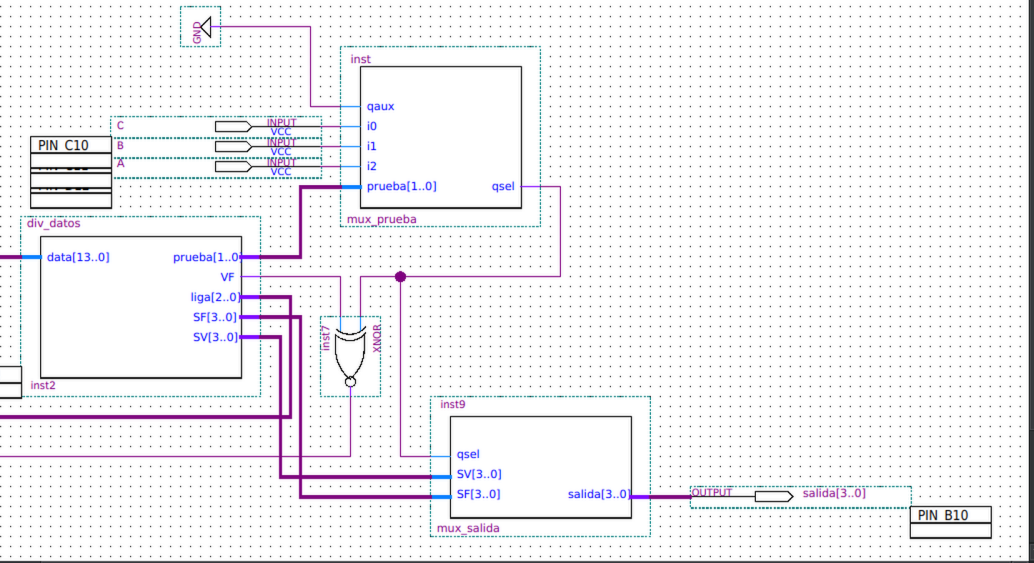
\includegraphics[width=0.90\linewidth]{diagramas_bloques_3.png}
\caption{Selector de prueba y lógica de selección de las salidas.}
\label{fig:bloques-3}
\end{figure}

\subsection{Módulos implementados en VHDL}

\paragraph{Registro e incrementador:} El registro conserva el estado presente. Su reinicio es asíncrono y activo en bajo; con \texttt{reset='0'} fuerza \texttt{000}, mientras que cada flanco ascendente carga el estado siguiente. El incrementador calcula permanentemente $N+1$.

\lstinputlisting[style=estiloVHDL,caption={Registro del estado presente.},label={lst:registro}]{code/registro.vhd}

\lstinputlisting[style=estiloVHDL,caption={Incrementador para obtener la dirección implícita $N+1$.},label={lst:incrementador}]{code/incrementador.vhd}

\paragraph{Multiplexor de control:} Este bloque forma el contador con carga: selecciona el valor incrementado cuando \texttt{carga=0} o la liga almacenada cuando \texttt{carga=1}.

\lstinputlisting[style=estiloVHDL,caption={Selección entre $N+1$ y la liga explícita $P$.},label={lst:mux-control}]{code/mux_control.vhd}

\paragraph{ROM y división de datos.} La ROM contiene ocho palabras de 14 bits. El bloque \texttt{div\_datos} separa los bits $[13:12]$ como prueba, el bit $[11]$ como $VF$, los bits $[10:8]$ como liga, $[7:4]$ como salida falsa y $[3:0]$ como salida verdadera.

\lstinputlisting[style=estiloVHDL,caption={ROM de $8\times14$ bits con el microprograma.},label={lst:rom}]{code/rom.vhd}

\lstinputlisting[style=estiloVHDL,caption={Separación de los campos de la palabra de 14 bits.},label={lst:div-datos}]{code/div_datos.vhd}

\paragraph{Selección de prueba y salidas.} El multiplexor de prueba convierte el código almacenado en la ROM en el valor de una de las entradas. El multiplexor de salida utiliza este mismo resultado para escoger el vector falso o verdadero.

\lstinputlisting[style=estiloVHDL,caption={Selección de $A$, $B$, $C$ o $QAUX$.},label={lst:mux-prueba}]{code/mux_prueba.vhd}

\lstinputlisting[style=estiloVHDL,caption={Selección de la salida falsa o verdadera.},label={lst:mux-salida}]{code/mux_salida.vhd}

\paragraph{Reloj por botón.} Para observar las transiciones en la tarjeta, el módulo \texttt{clk\_buttom} genera un pulso controlado a partir del reloj de la FPGA y de un botón. Así se evita recorrer varios estados antes de poder identificar visualmente las salidas.

\lstinputlisting[style=estiloVHDL,caption={Acondicionamiento del reloj mediante botón.},label={lst:clk-button}]{code/clk_buttom.vhd}

\section{Simulación}

La simulación en \texttt{Multisim} fue con una señal de reloj preestablecida, con \texttt{reset=1} y diferentes combinaciones para $A$, $B$ y $C$. Las señales \texttt{edop} y \texttt{salida} permiten relacionar el estado presente con la palabra leída de la ROM. Como el registro cambia únicamente en el flanco ascendente, \texttt{edop} permanece estable entre flancos aunque las entradas se modifiquen.

En la Figura[\ref{fig:simulacion-1}] se observan recorridos como \texttt{000}$\rightarrow$\texttt{100}$\rightarrow$\texttt{000} y \texttt{000}$\rightarrow$\texttt{001}$\rightarrow$\texttt{011}$\rightarrow$\texttt{000}. El primer recorrido ocurre cuando $A=0$, por lo que se carga la liga de $E_0$ hacia $E_4$. El segundo comienza con $A=1$, que selecciona la dirección implícita $N+1=001$; posteriormente, con $B=0$, se carga \texttt{011}.

\begin{figure}[H]
\centering
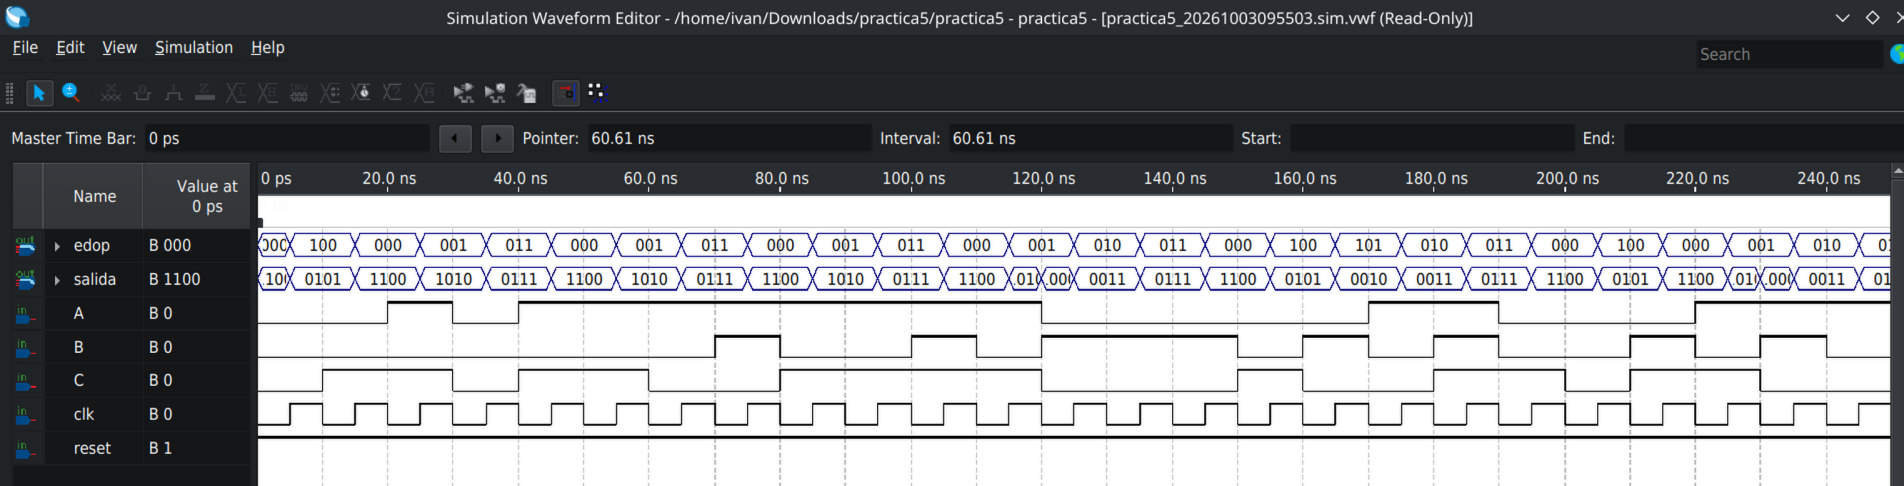
\includegraphics[width=\linewidth]{simulacion_1.png}
\caption{Primera parte de la simulación funcional del direccionamiento implícito.}
\label{fig:simulacion-1}
\end{figure}

La Figura[\ref{fig:simulacion-2}] incluye secuencias que atraviesan la rama derecha de la carta ASM. Desde \texttt{100}, si $C=0$, no se carga la liga porque $C\neq VF$ y el contador avanza a \texttt{101}, en $E_5$, $QAUX=0$ coincide con $VF=0$ y se carga la liga \texttt{010}. Después, $E_2$ utiliza nuevamente el avance implícito para llegar a \texttt{011}, y $E_3$ carga la liga \texttt{000}.

\begin{figure}[H]
\centering
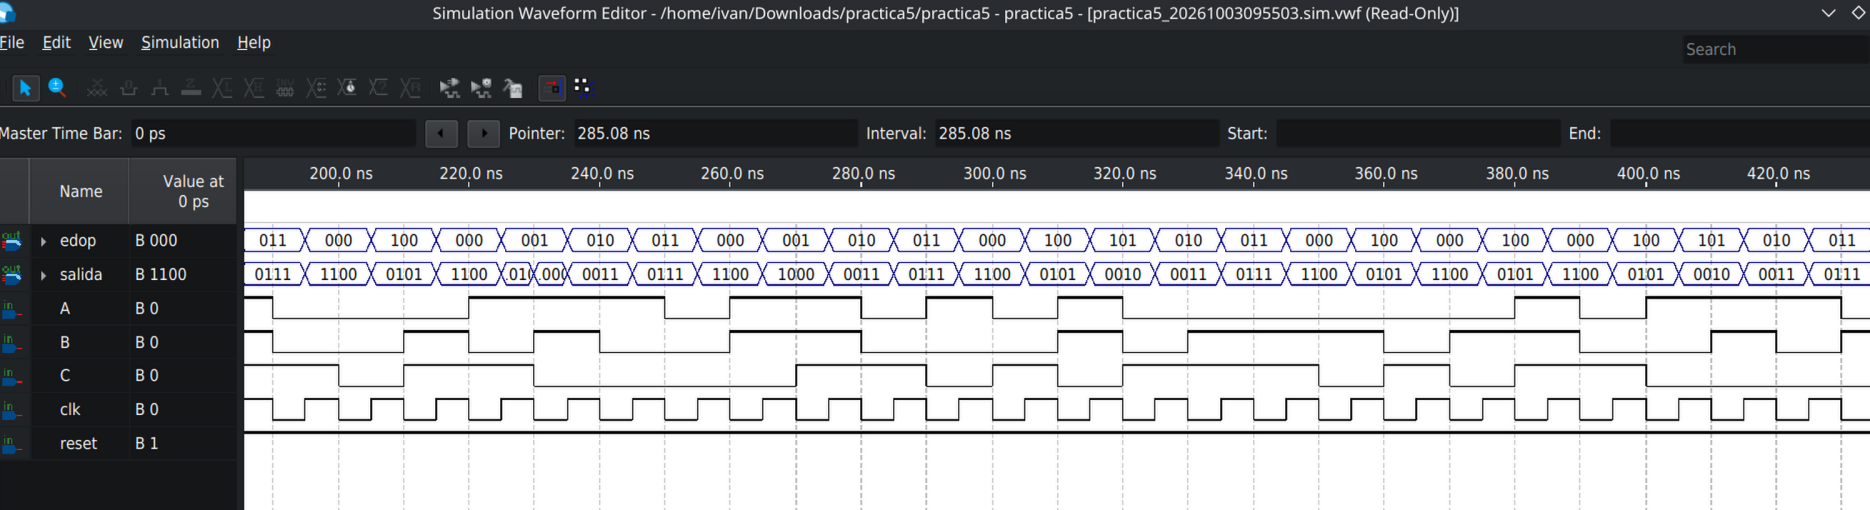
\includegraphics[width=\linewidth]{simulacion_2.png}
\caption{Transiciones mediante la liga explícita y la dirección implícita $N+1$.}
\label{fig:simulacion-2}
\end{figure}

En la parte final, mostrada en la Figura[\ref{fig:simulacion-3}], se repiten distintas rutas al modificar las entradas. Los valores de \texttt{salida} coinciden con el programa implementado: \texttt{1100} en $E_0$, \texttt{1010} o \texttt{1000} en $E_1$, \texttt{0011} en $E_2$, \texttt{0111} en $E_3$, \texttt{0101} en $E_4$ y \texttt{0010} en $E_5$. Esto verifica tanto la selección de la liga como la selección de la salida correspondiente a cada rama.

\begin{figure}[H]
\centering
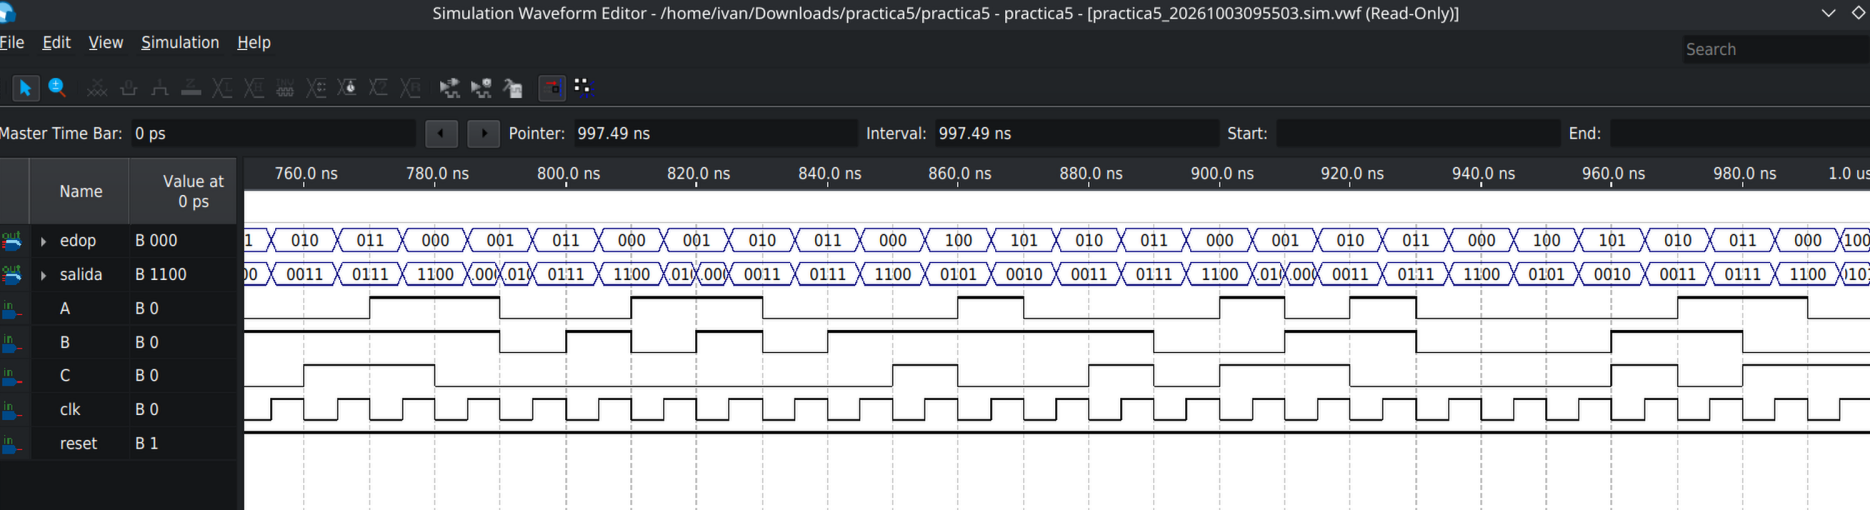
\includegraphics[width=\linewidth]{simulacion_3.png}
\caption{Parte final de la simulación, con diferentes recorridos de la carta ASM.}
\label{fig:simulacion-3}
\end{figure}

\section{Resultados en la tarjeta FPGA}

El diseño se implementó en la tarjeta  de desarrollo DE10-Lite. Los tres LEDs asignados a \texttt{edop} muestran el código del estado presente y cuatro LEDs adicionales representan \texttt{salida}. Las fotografías permiten contrastar directamente los valores físicos con la Tabla~\ref{tab:memoria}.

\begin{figure}[H]
\centering
\begin{subfigure}[b]{0.45\linewidth}
  \centering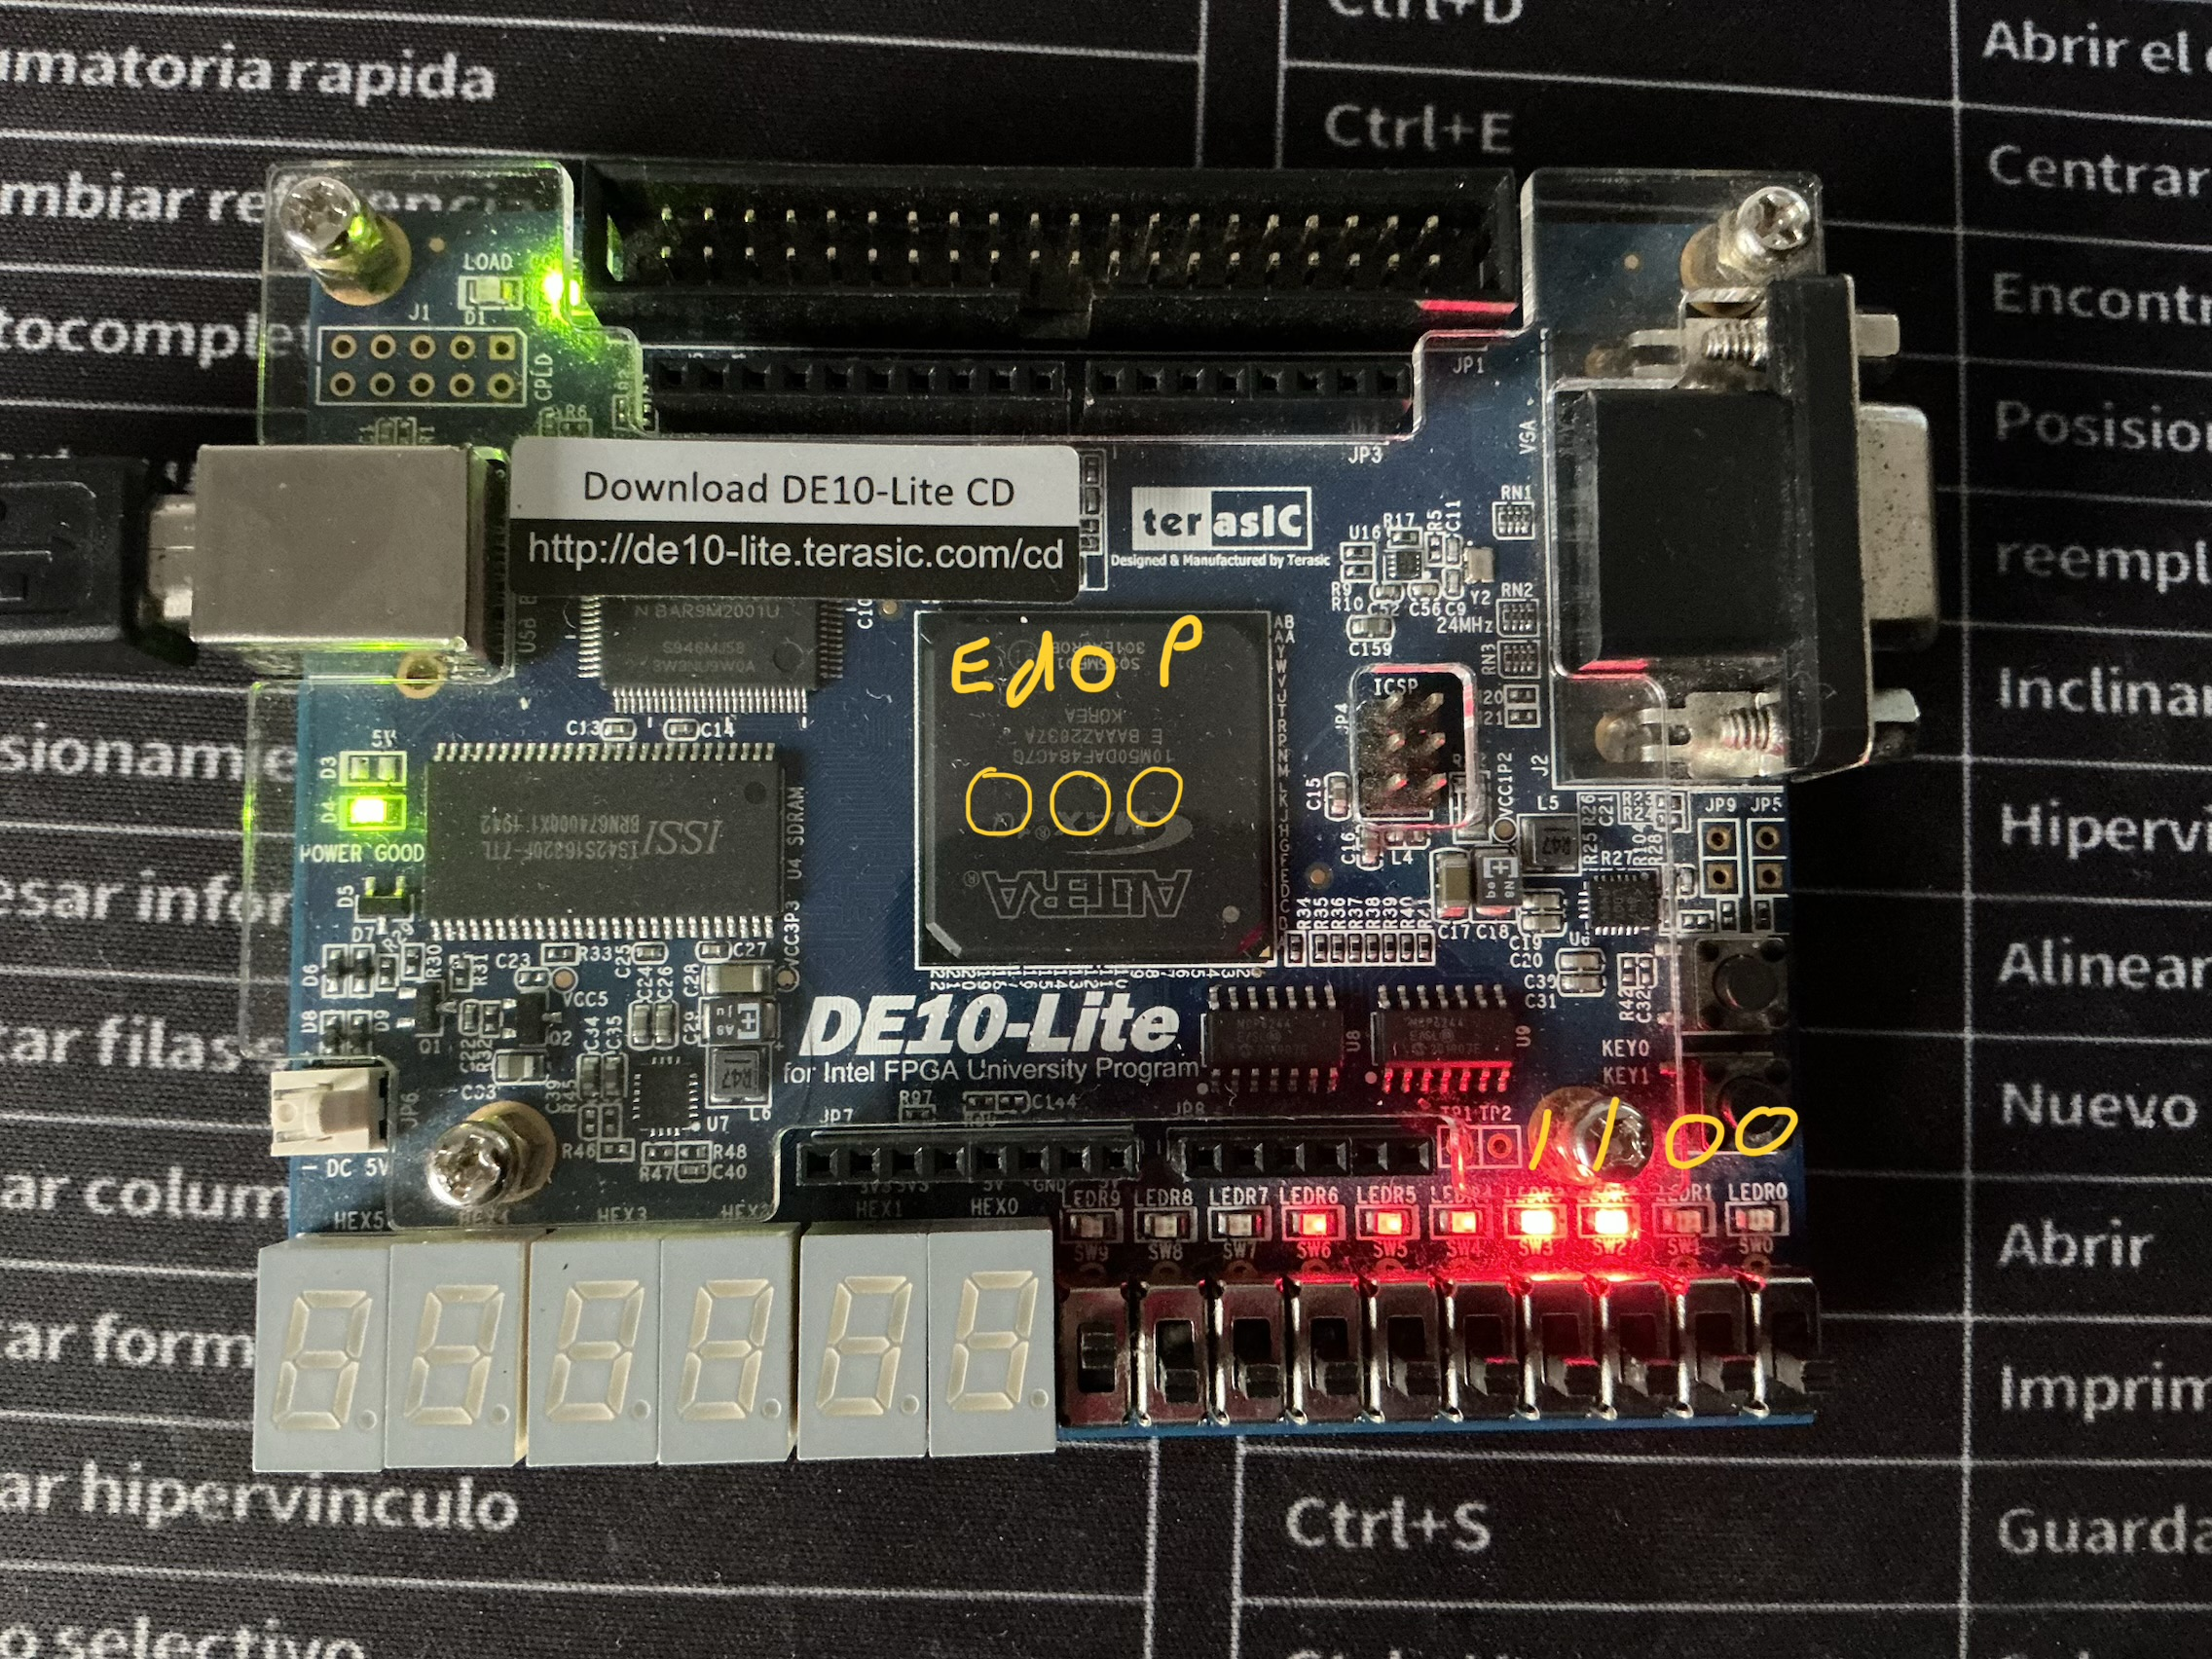
\includegraphics[width=\linewidth]{est0.jpeg}
  \caption{$E_0=000$, salida \texttt{1100}.}
\end{subfigure}\hfill
\begin{subfigure}[b]{0.45\linewidth}
  \centering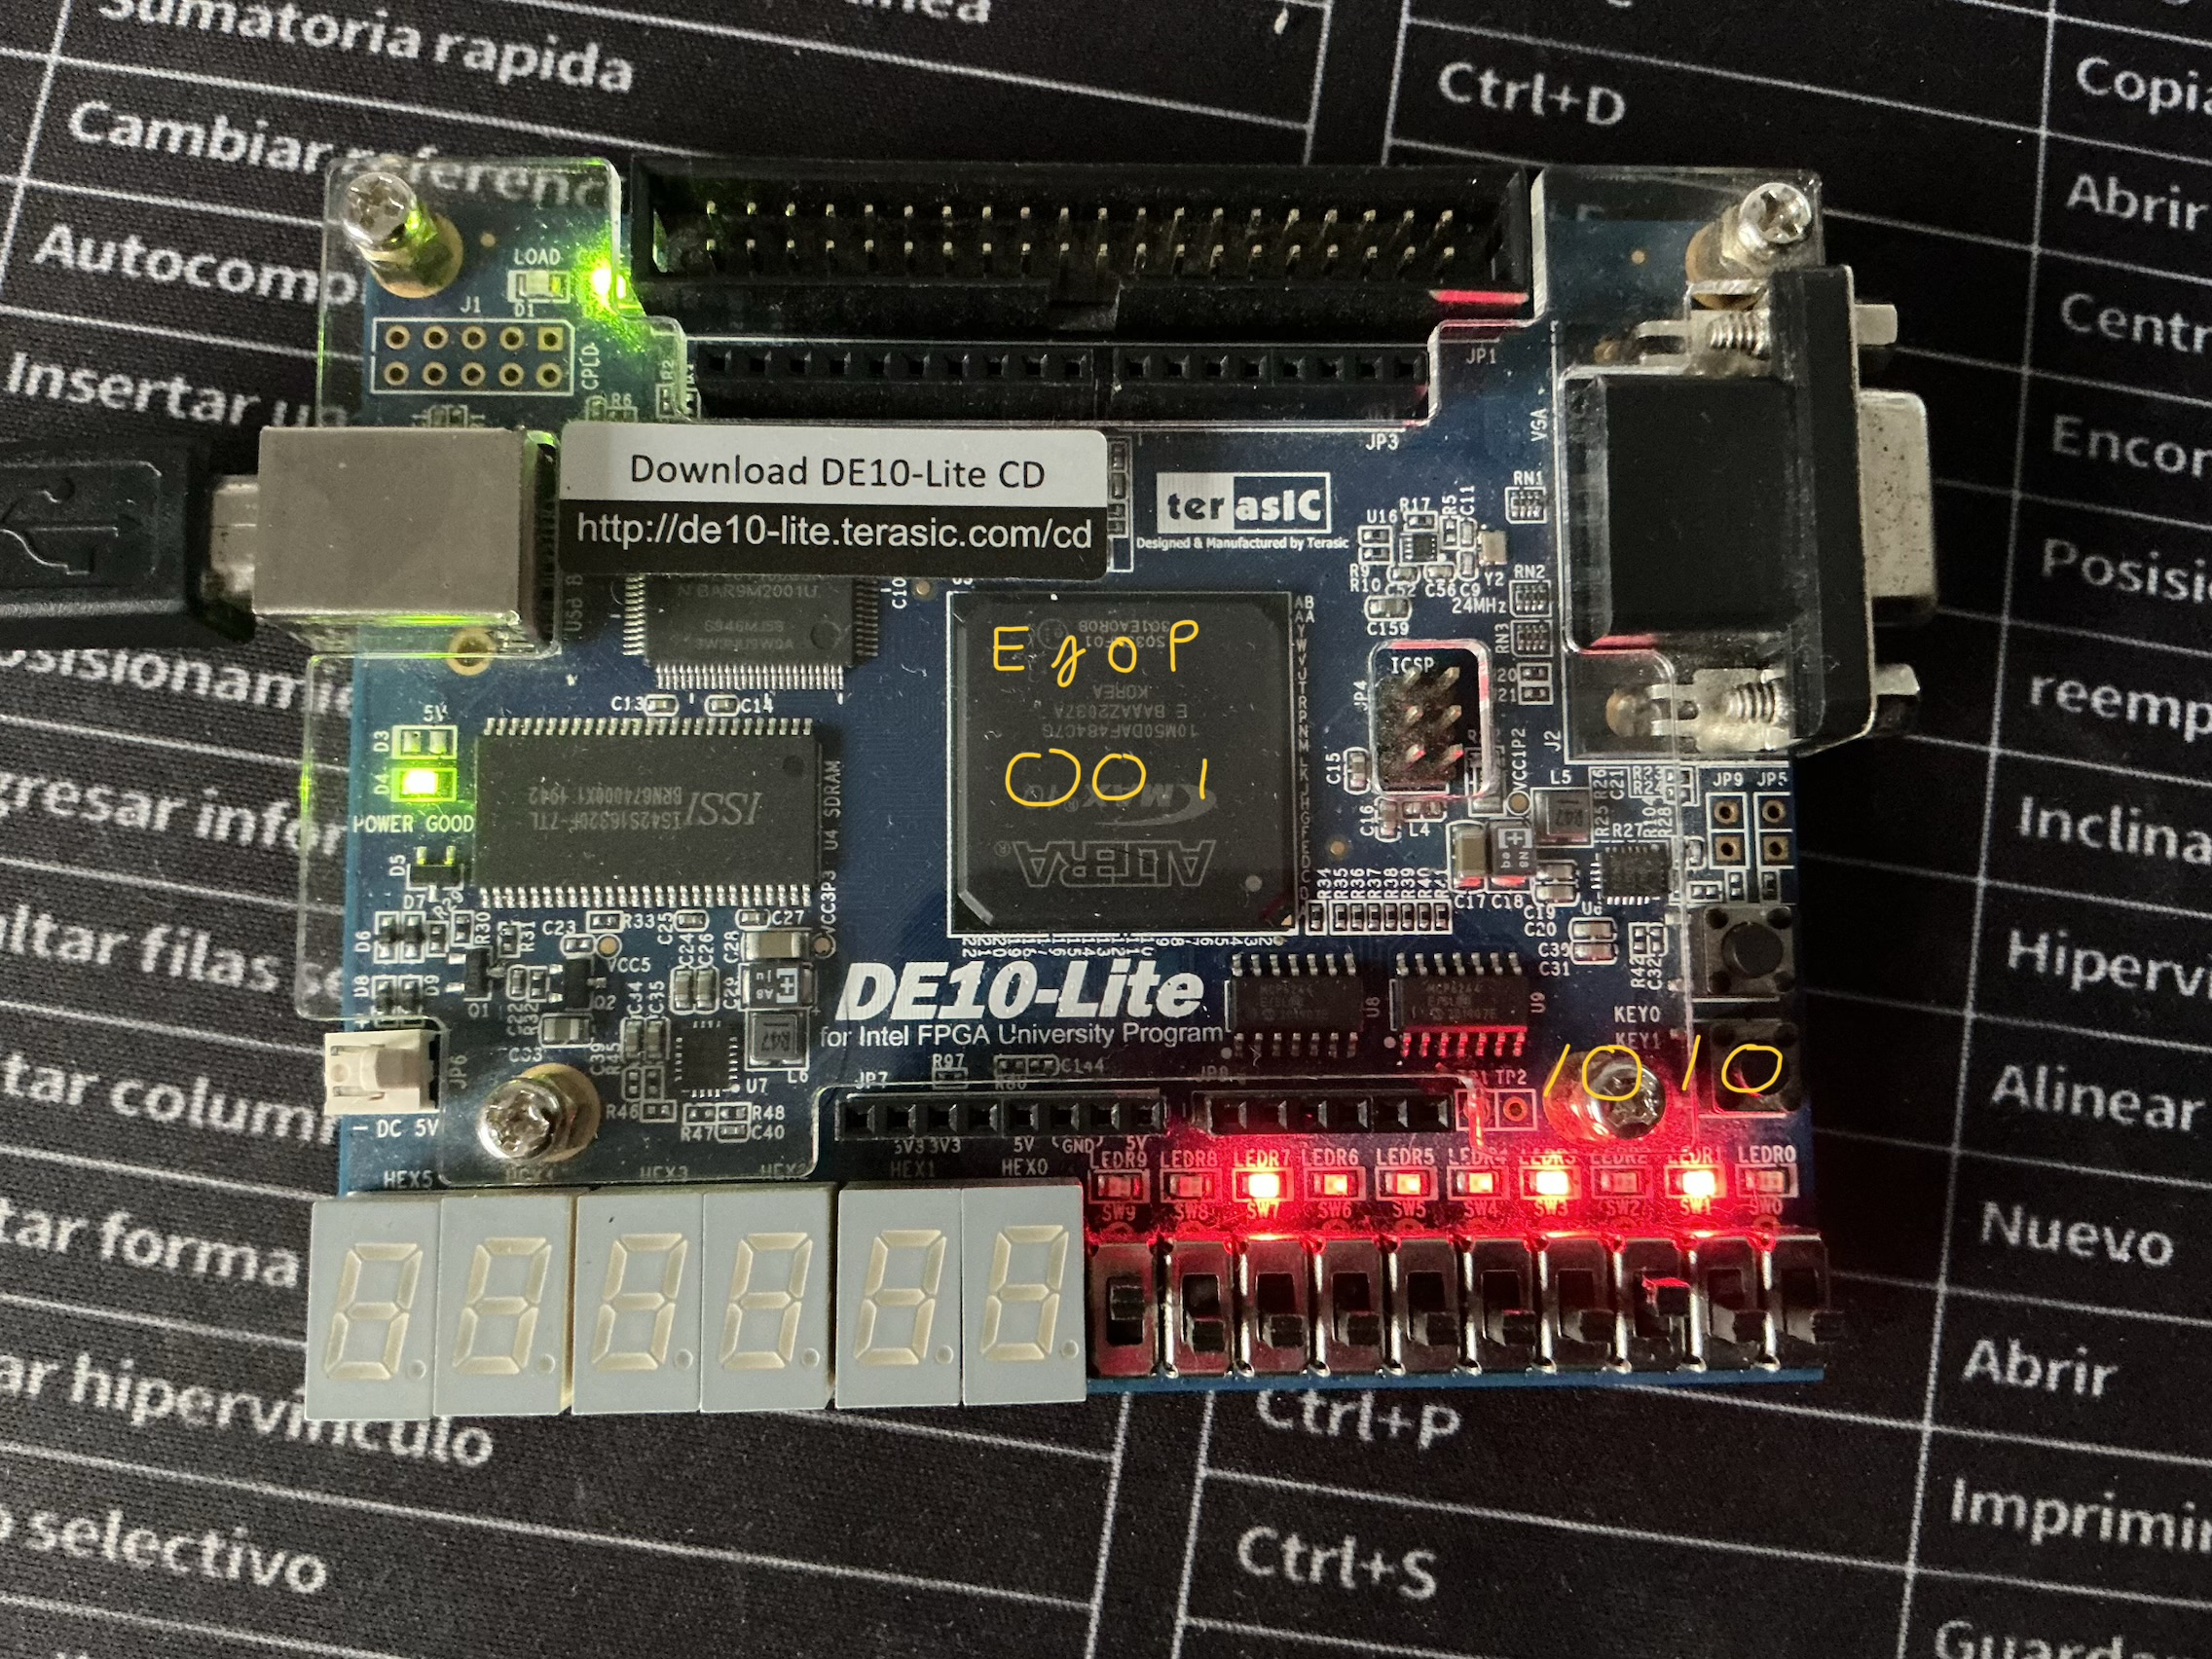
\includegraphics[width=\linewidth]{est1_b_0.jpeg}
  \caption{$E_1=001$ con $B=0$, salida \texttt{1010}.}
\end{subfigure}
\caption{Comprobación física de $E_0$ y de la rama falsa de $E_1$.}
\label{fig:fpga-01a}
\end{figure}

\begin{figure}[H]
\centering
\begin{subfigure}[b]{0.45\linewidth}
  \centering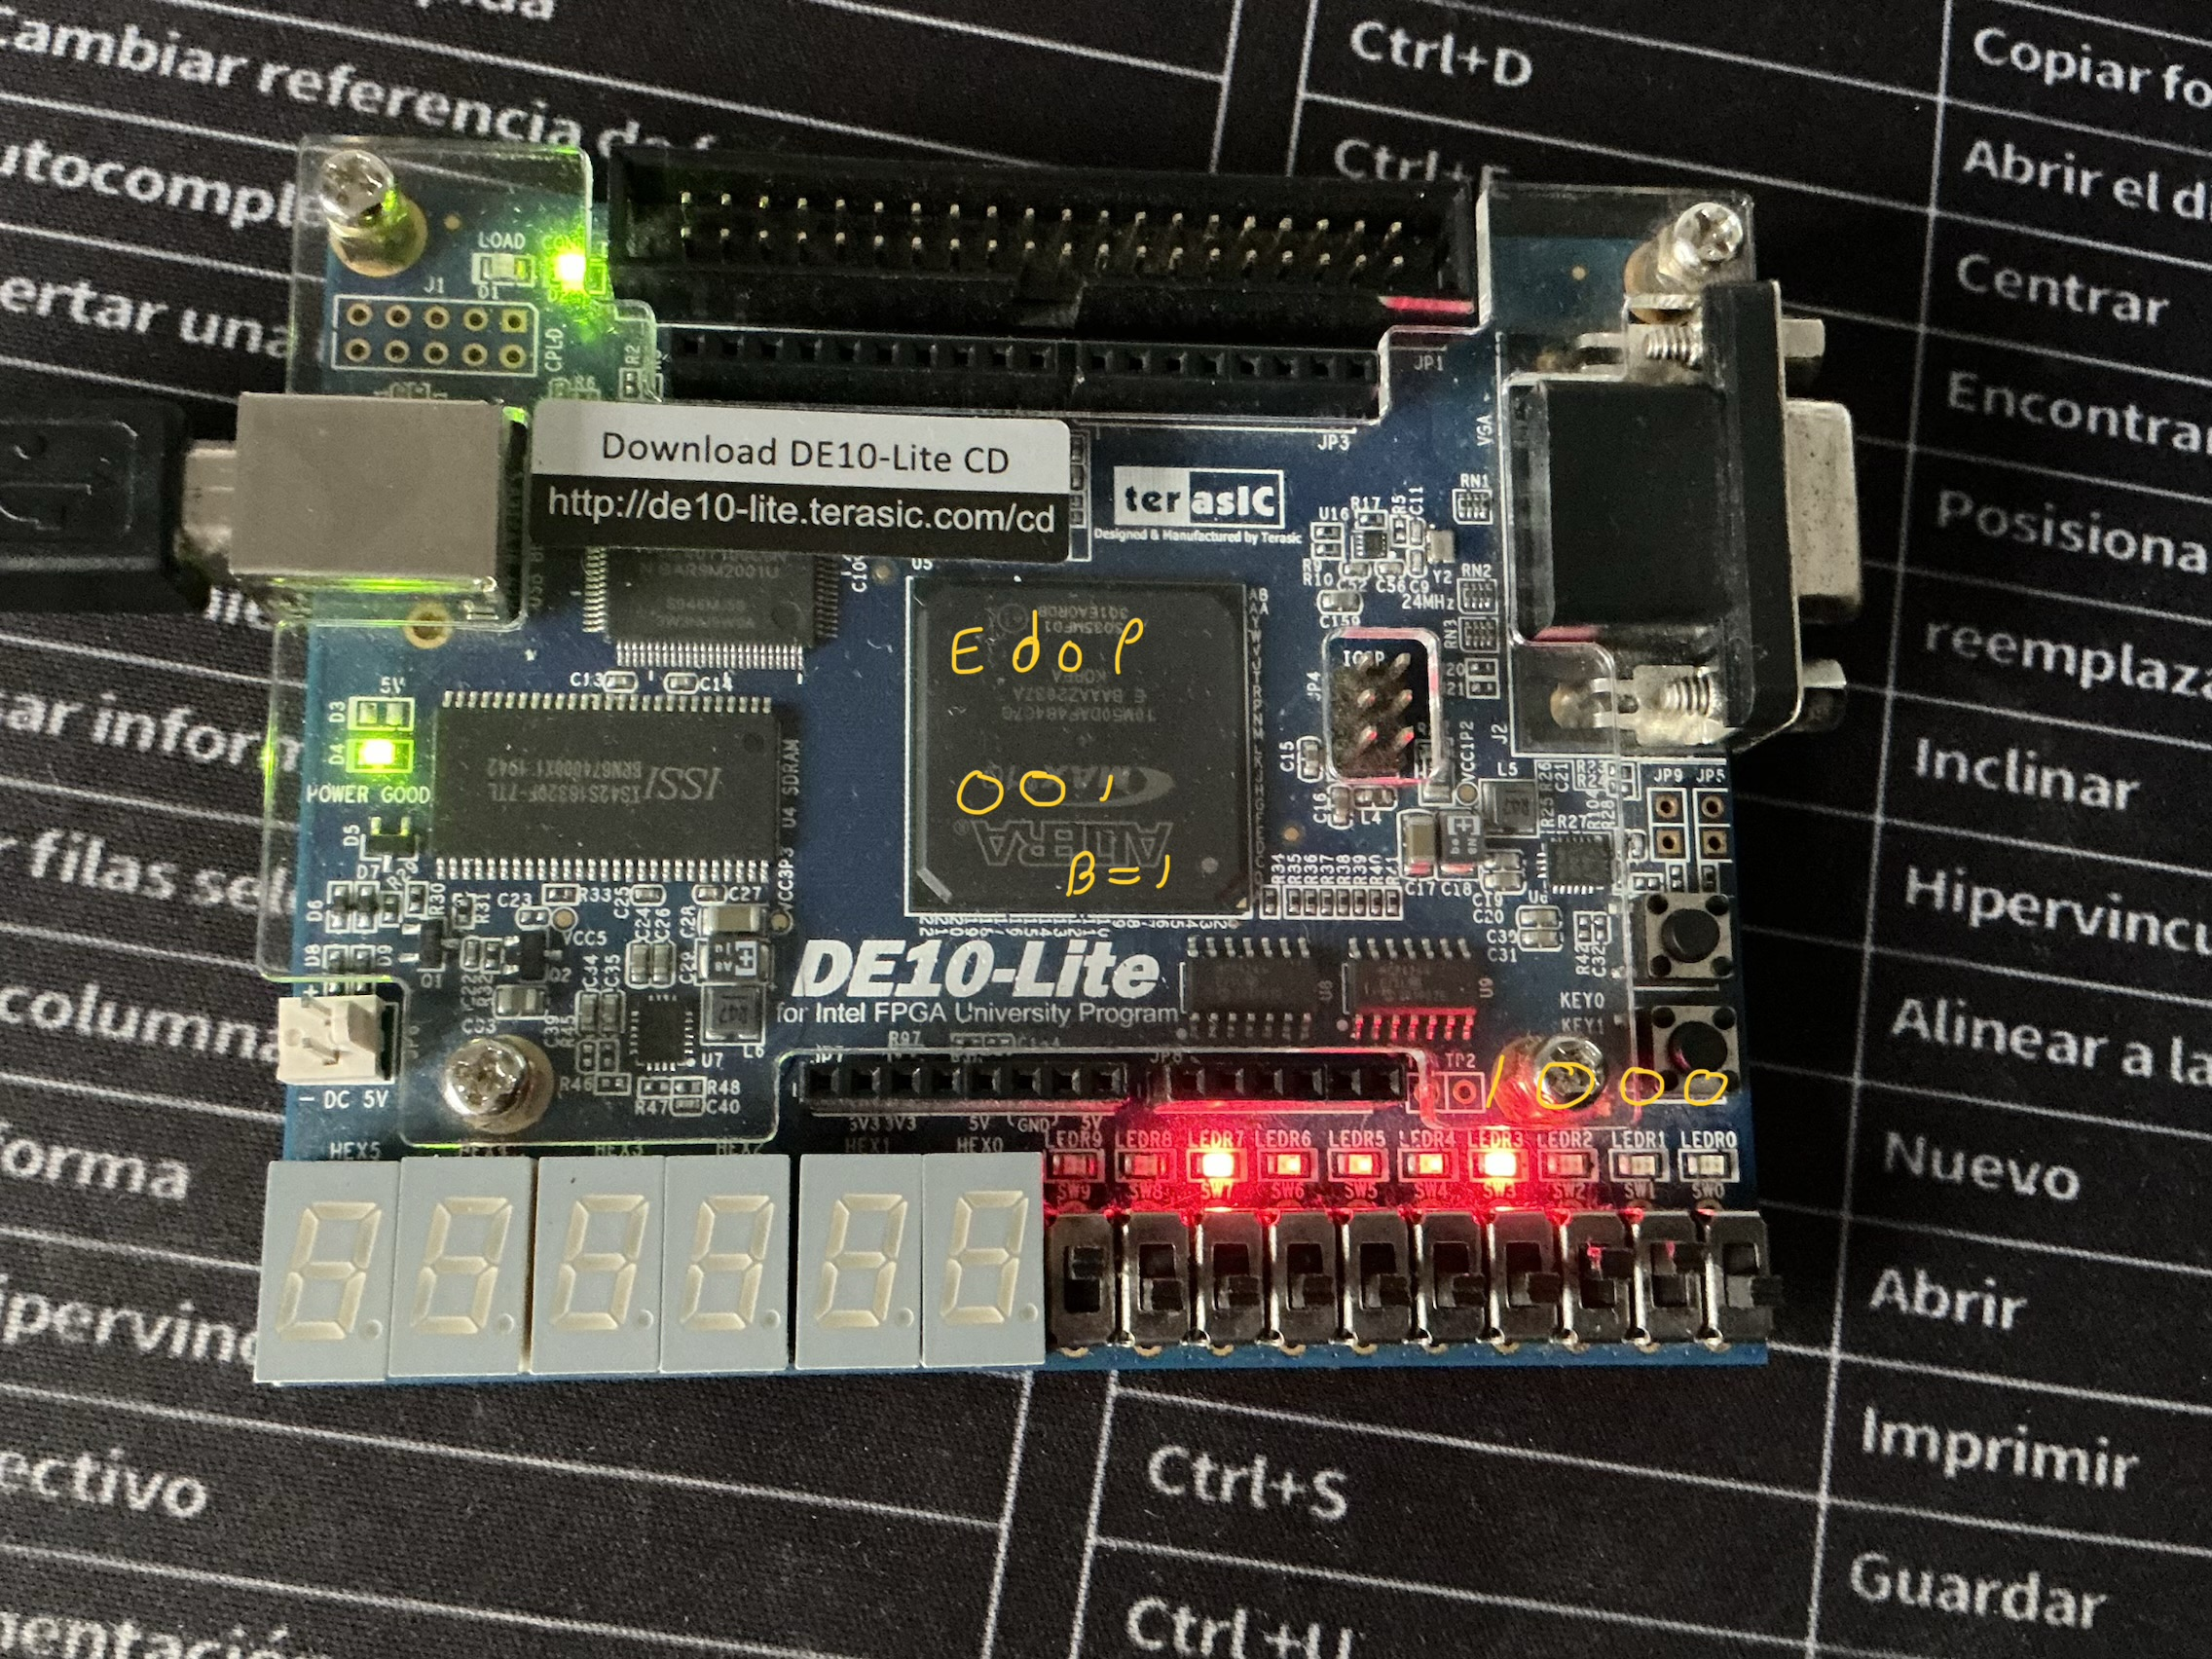
\includegraphics[width=\linewidth]{est1_b_1.jpeg}
  \caption{$E_1=001$ con $B=1$, salida \texttt{1000}.}
\end{subfigure}\hfill
\begin{subfigure}[b]{0.45\linewidth}
  \centering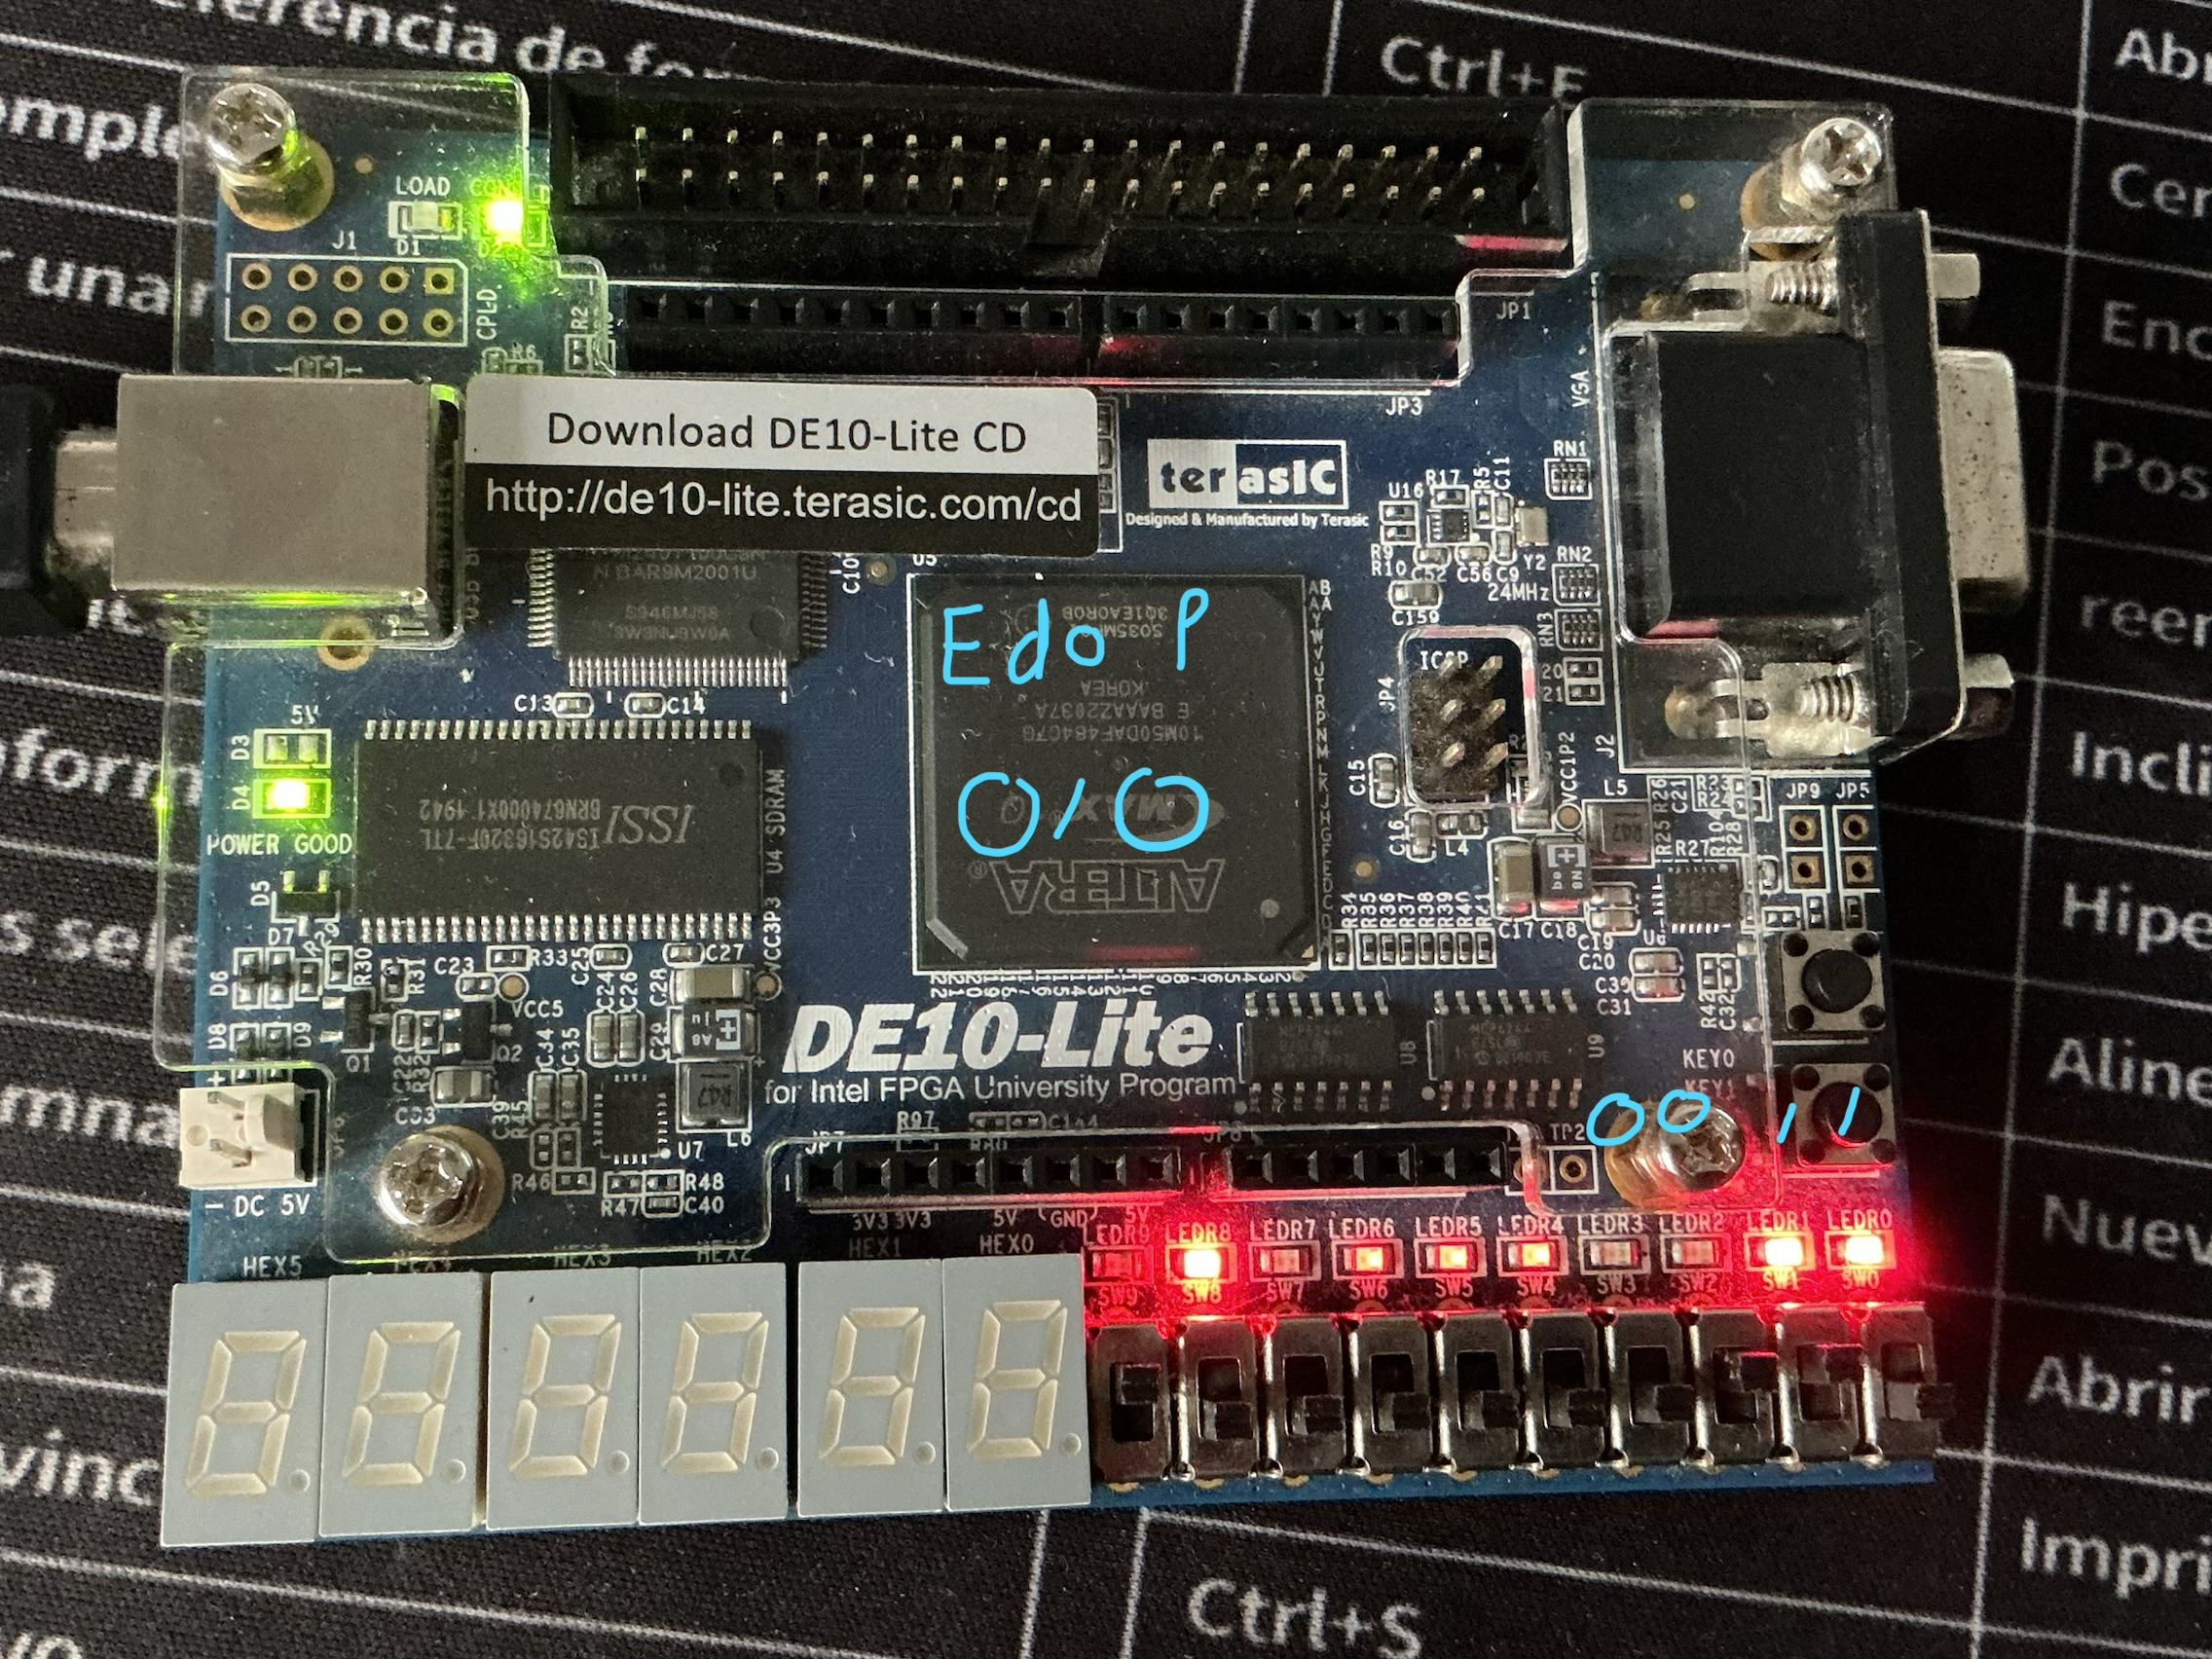
\includegraphics[width=\linewidth]{est2.jpeg}
  \caption{$E_2=010$, salida \texttt{0011}.}
\end{subfigure}
\caption{Rama verdadera de $E_1$ y evidencia del estado $E_2$.}
\label{fig:fpga-12}
\end{figure}

\begin{figure}[H]
\centering
\begin{subfigure}[b]{0.45\linewidth}
  \centering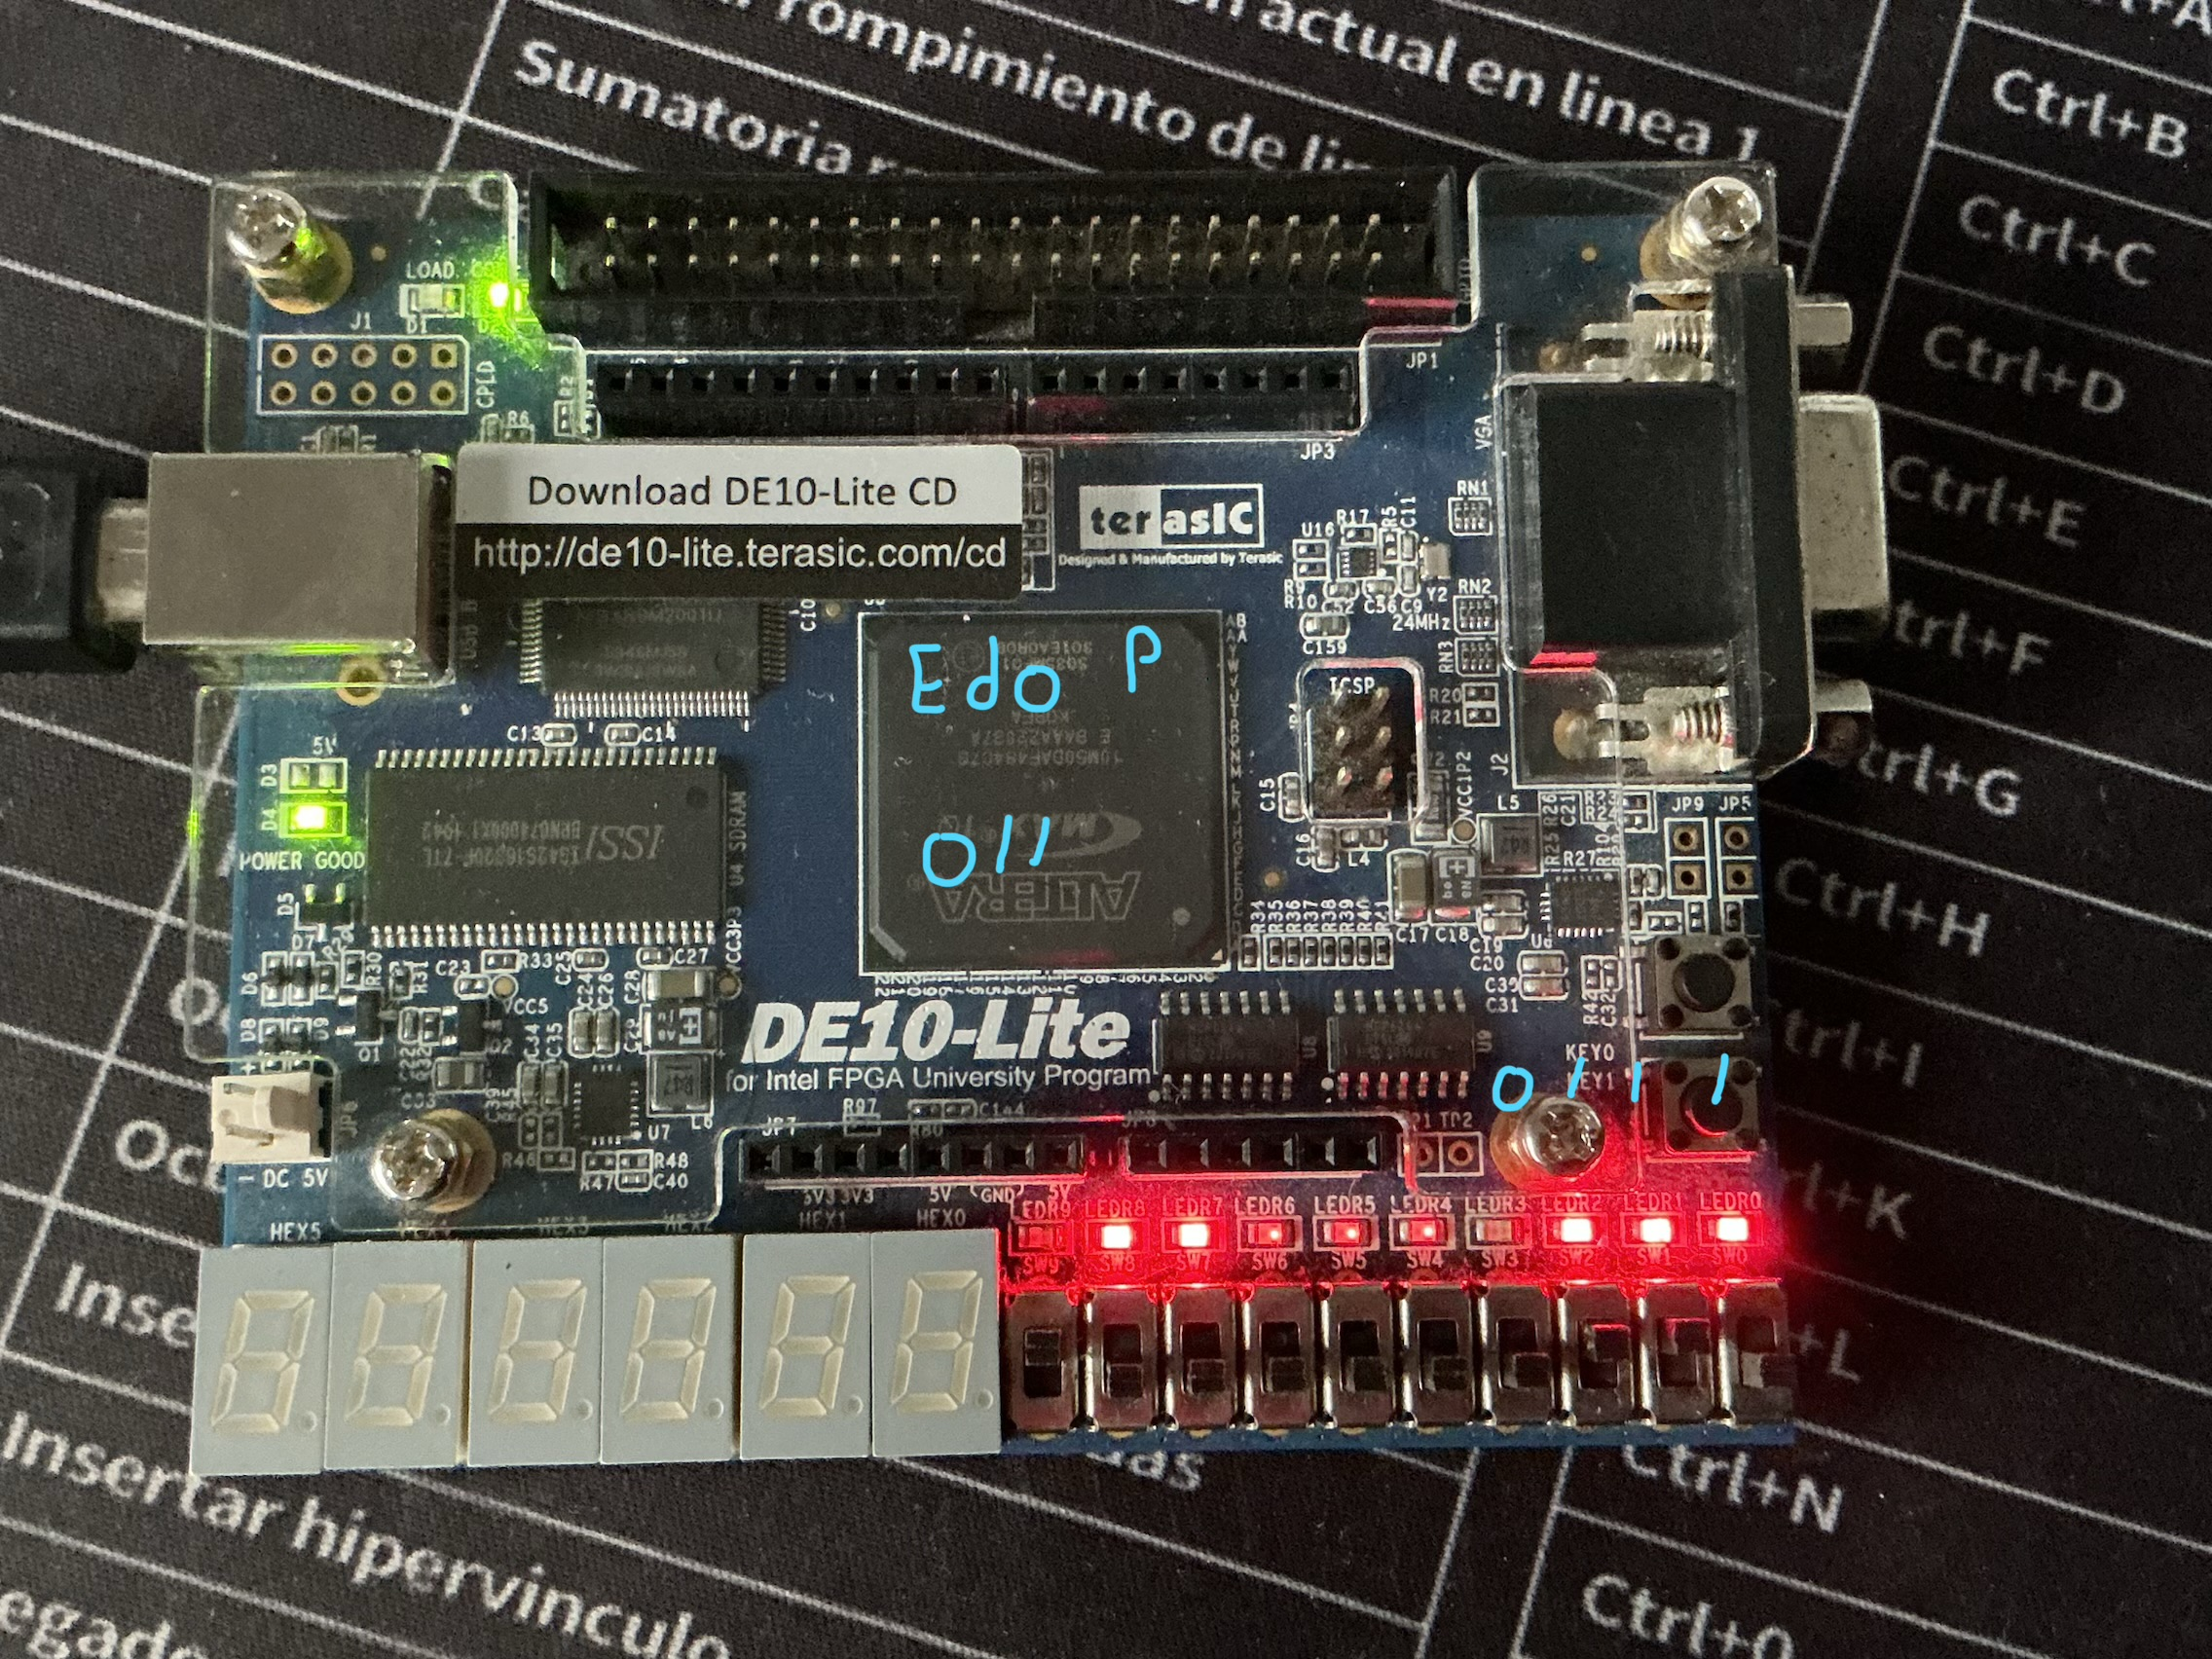
\includegraphics[width=\linewidth]{est3.jpeg}
  \caption{$E_3=011$, salida \texttt{0111}.}
\end{subfigure}\hfill
\begin{subfigure}[b]{0.45\linewidth}
  \centering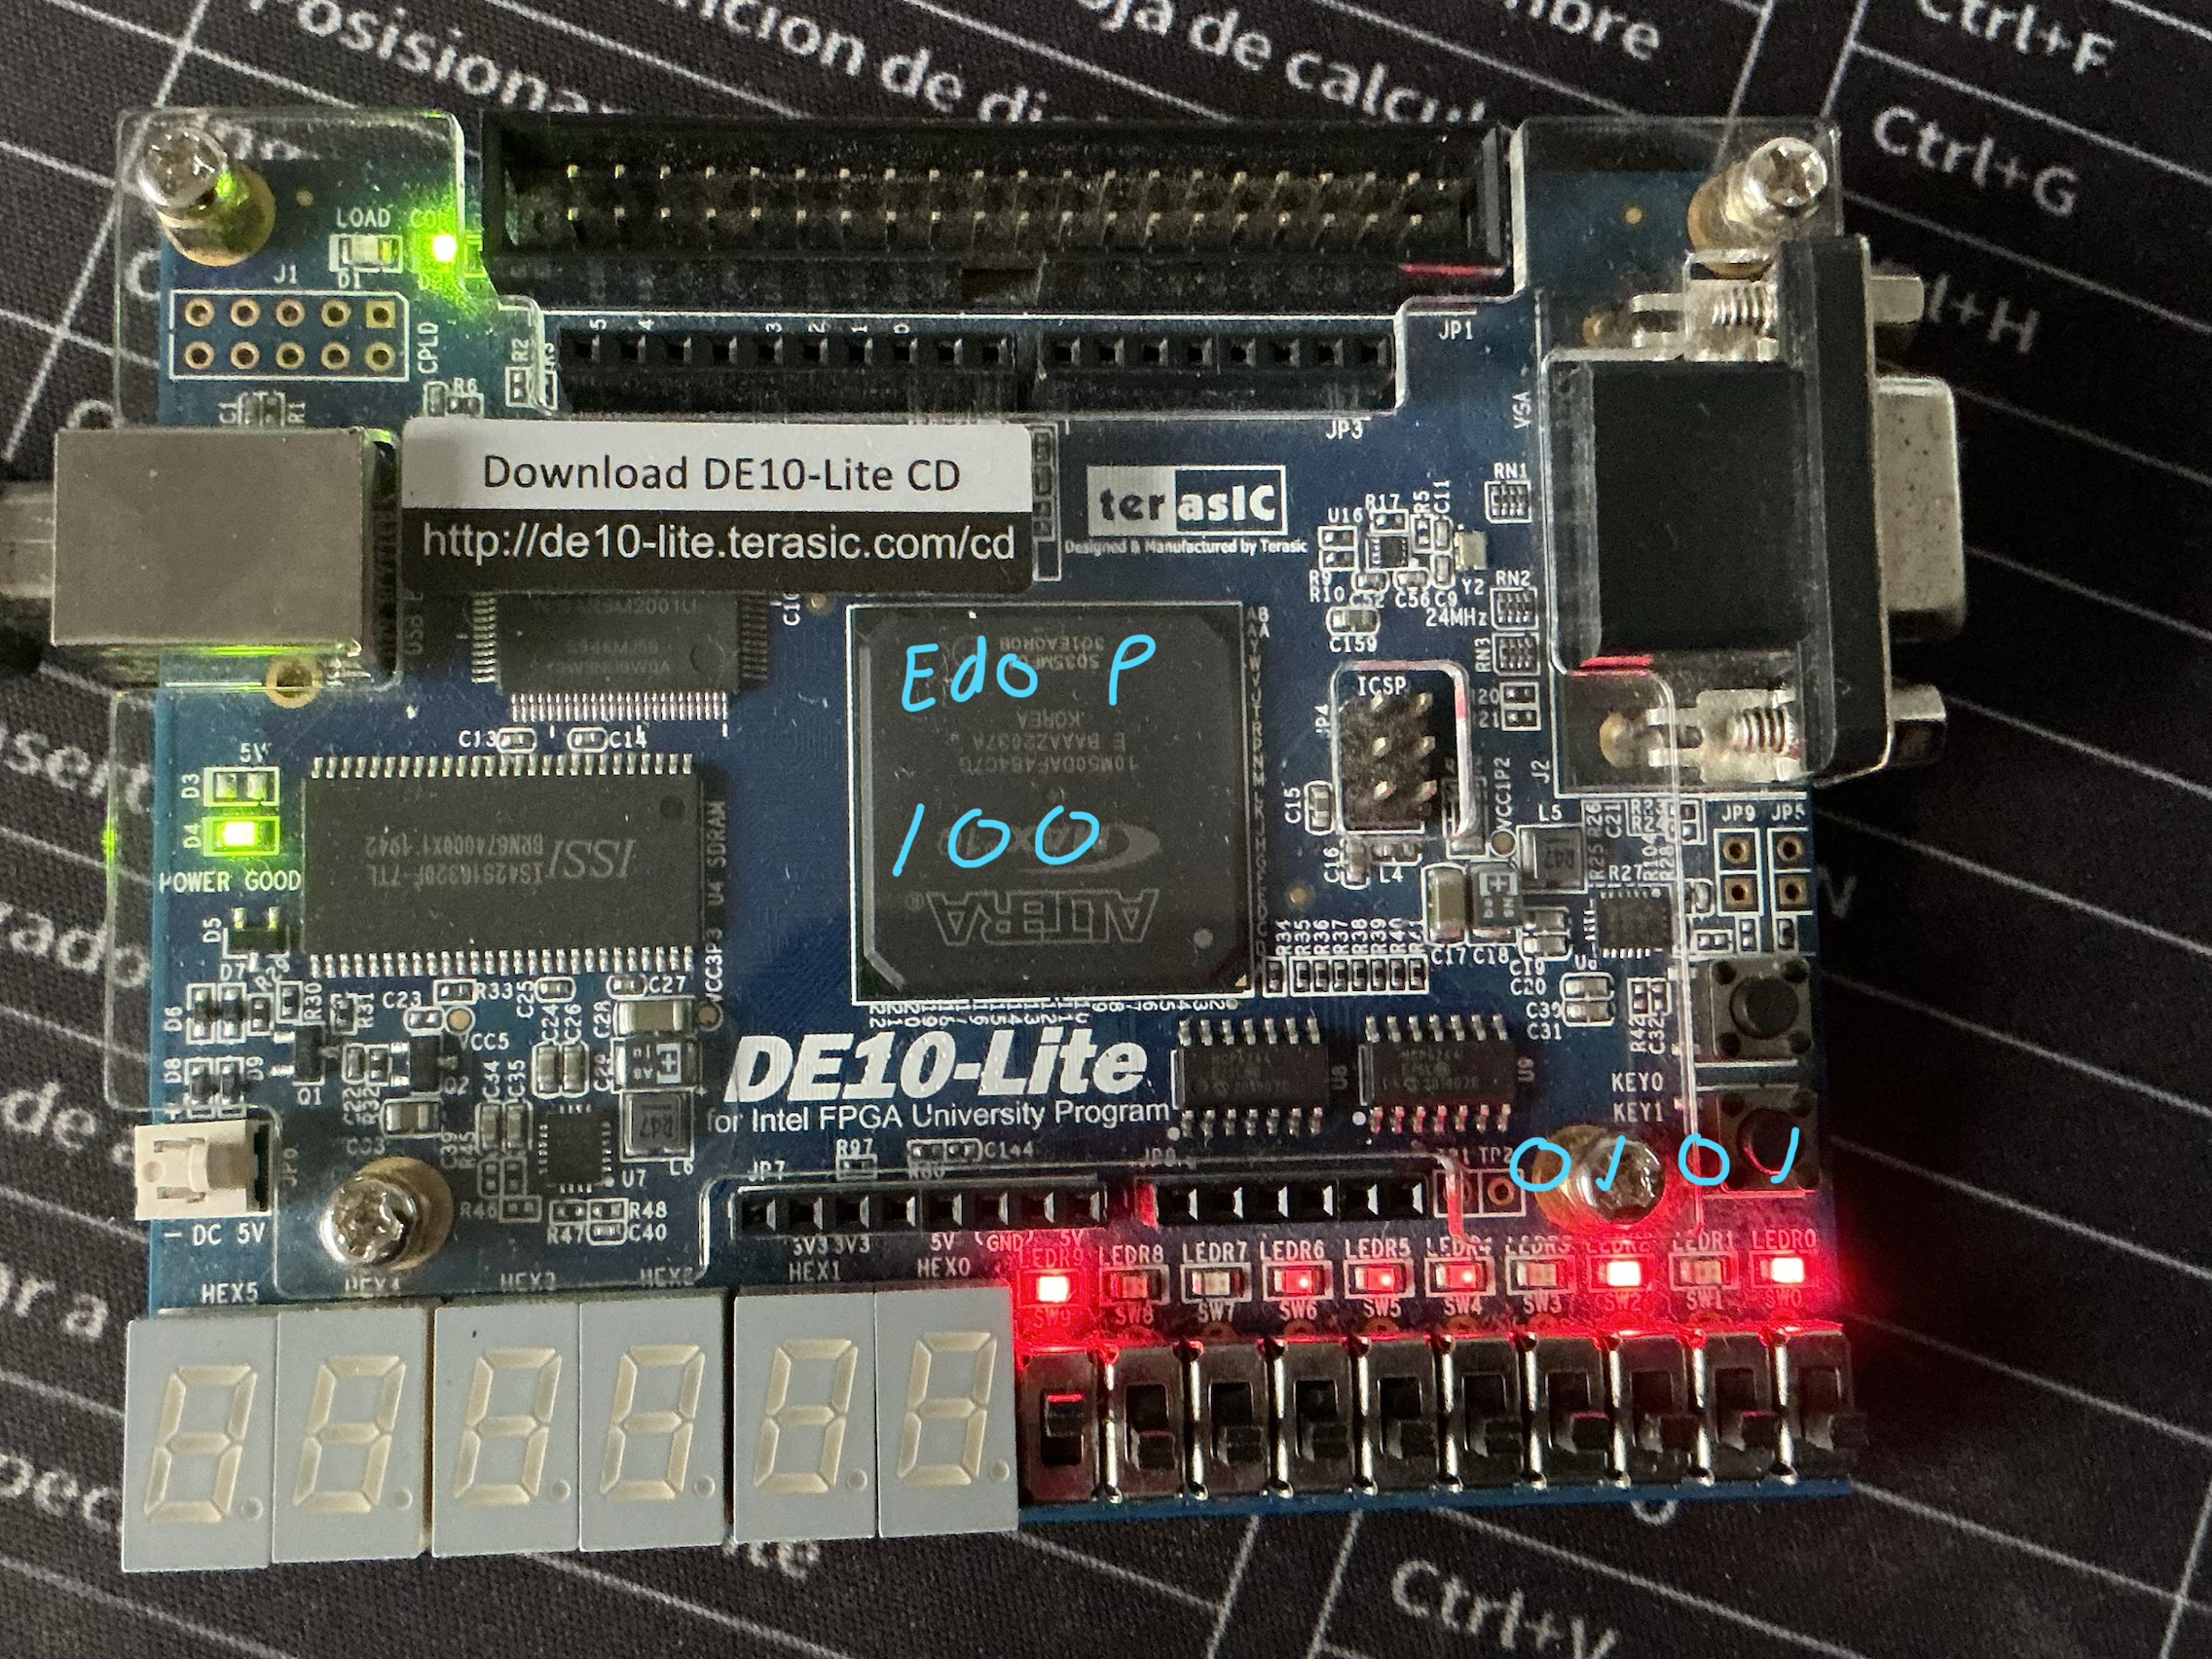
\includegraphics[width=\linewidth]{est4.jpeg}
  \caption{$E_4=100$, salida \texttt{0101}.}
\end{subfigure}
\caption{Comprobación física de los estados $E_3$ y $E_4$.}
\label{fig:fpga-34}
\end{figure}

\begin{figure}[H]
\centering
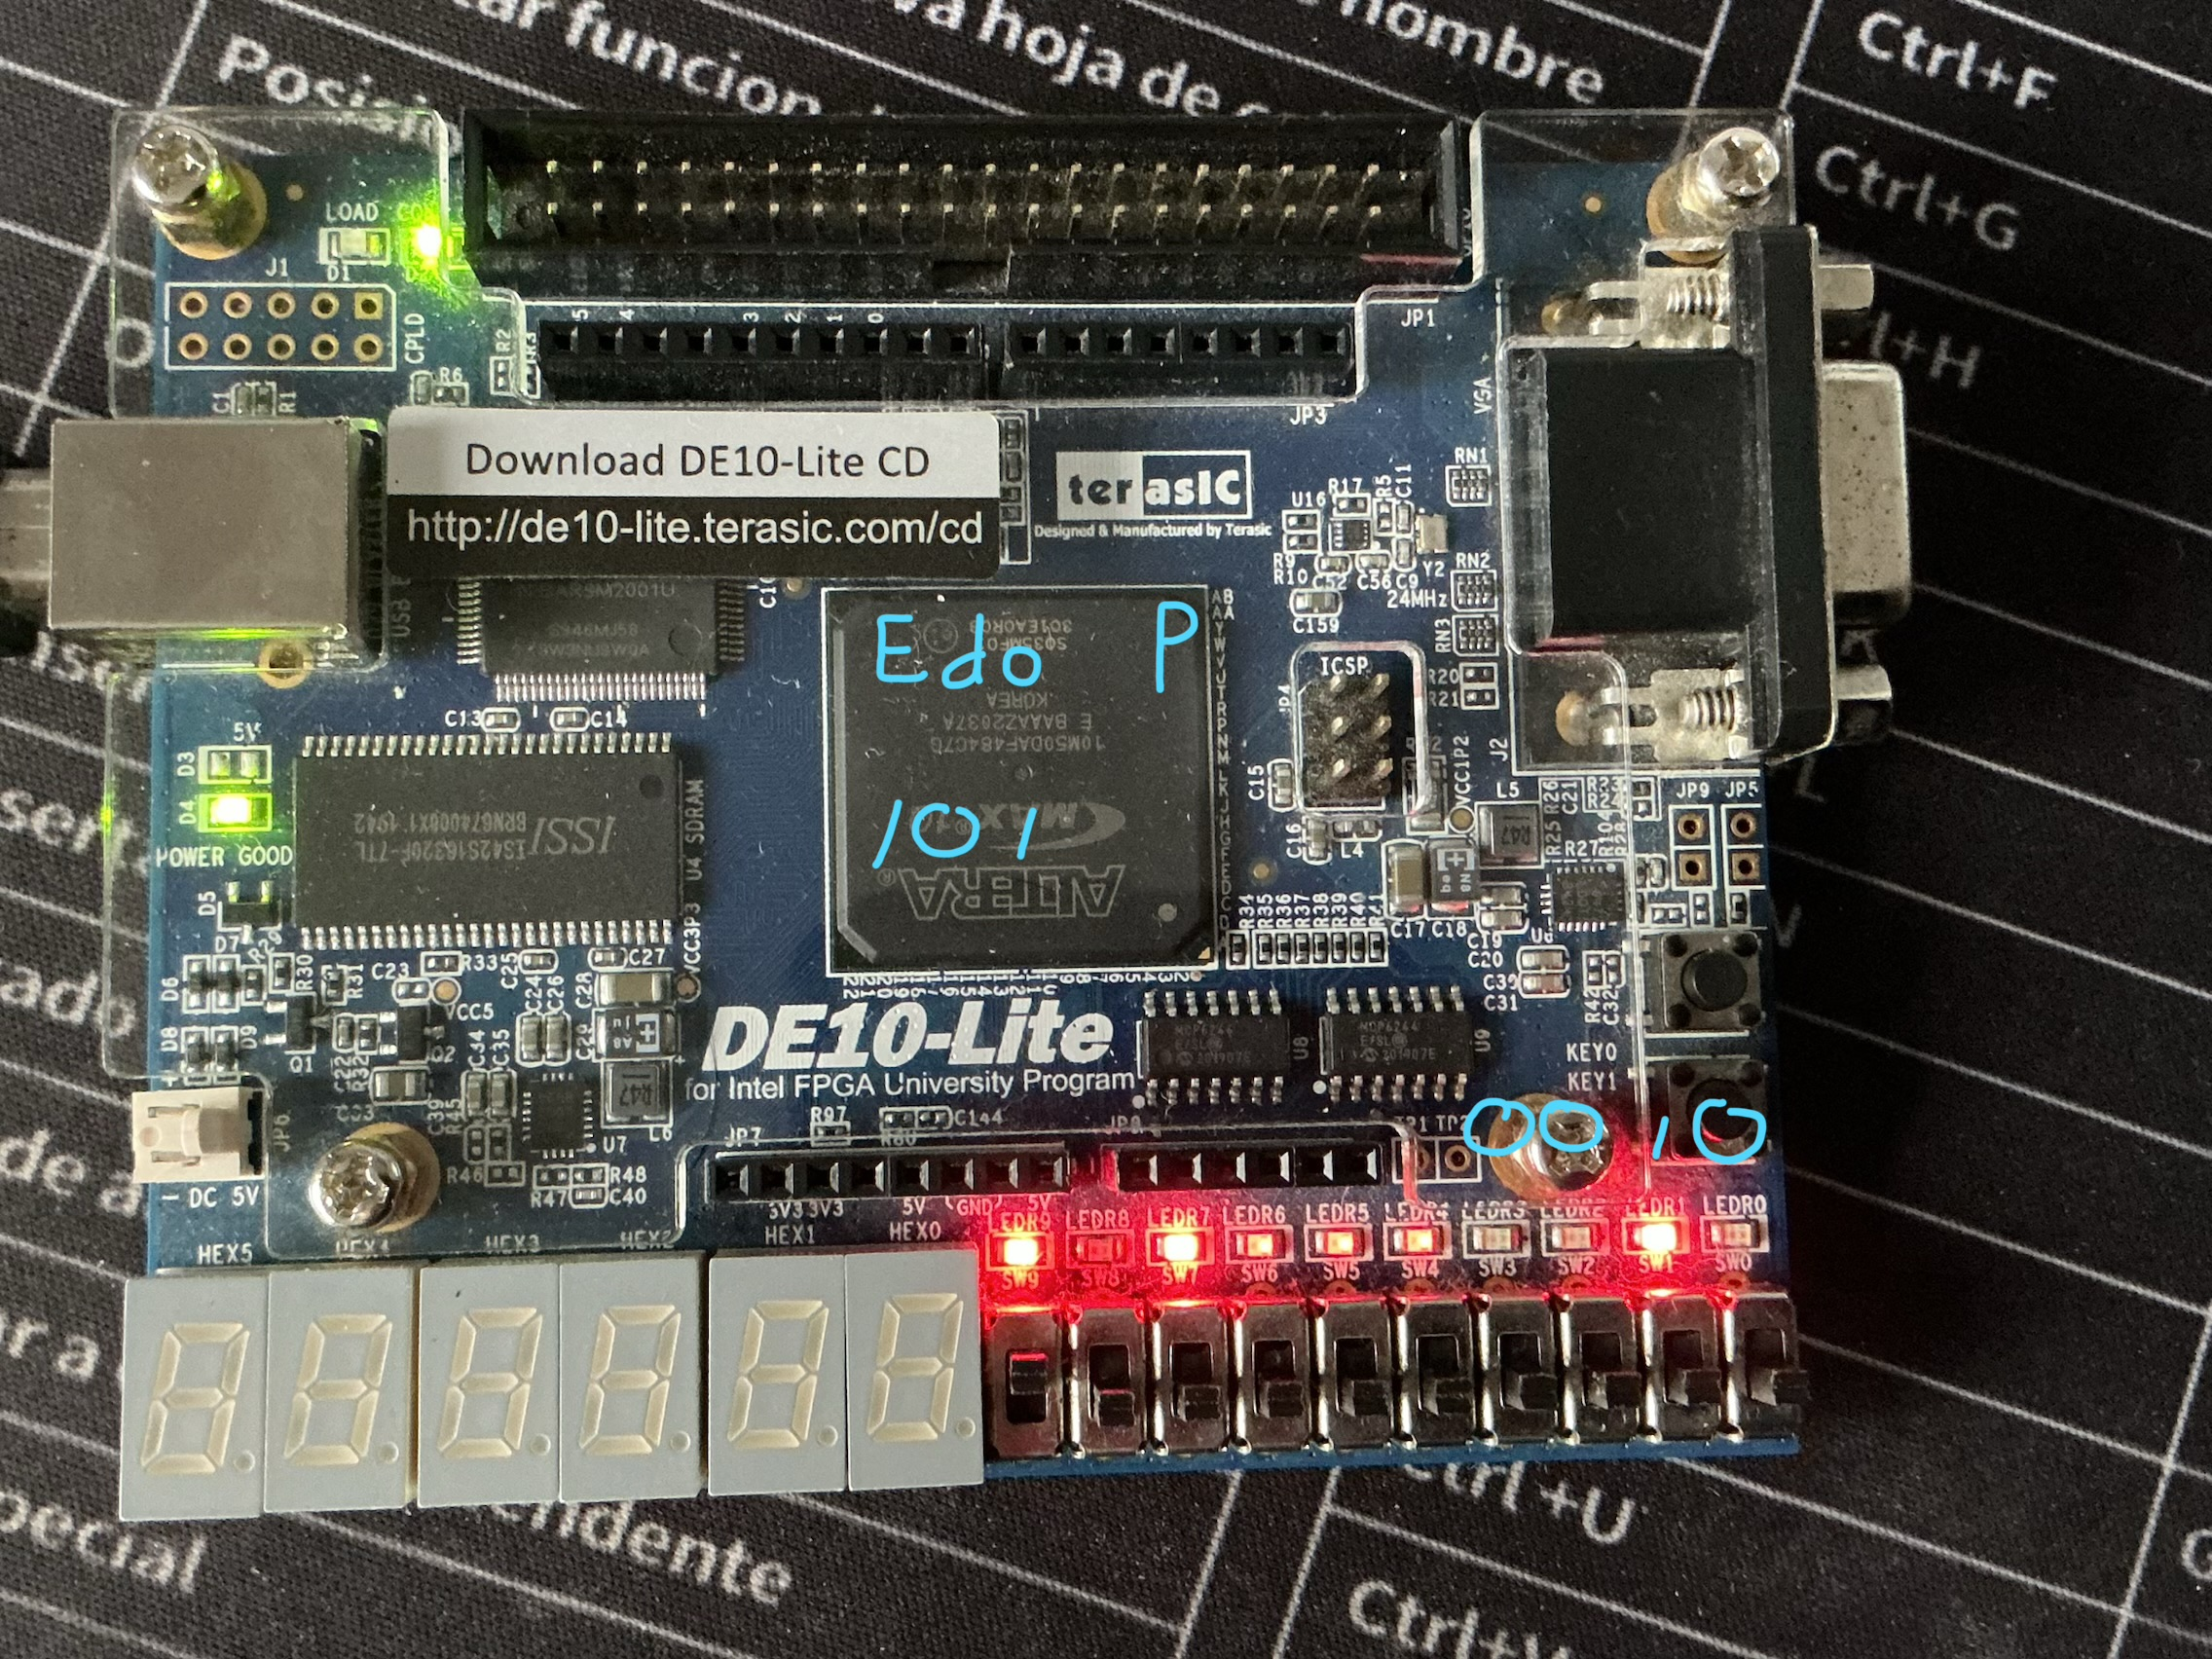
\includegraphics[width=0.45\linewidth]{est5.jpeg}
\caption{Estado $E_5=101$ con salida \texttt{0010}.}
\label{fig:fpga-5}
\end{figure}

Las implementación física confirmo que el contador avanza a $N+1$ cuando la entrada seleccionada es diferente de $VF$ y carga la liga almacenada cuando ambos valores coinciden. También se comprobó que el reinicio activo en bajo devuelve la máquina al estado \texttt{000} y que el pulso de reloj permite avanzar un estado a la vez.

\clearpage
\section{Conclusión}

\paragraph{Percival Ulises Espinoza Matamoros.} A partir de la implementación de la máquina de estados con direccionamiento implícito, comprendí el funcionamiento del direccionamiento implícito, el cuál permite reducir el tamaño de la memoria al aprovechar la secuencia de estados siempre y cuando se cumpla la regla $N$, $N+1$, $P$. La simulación y la implementación física me permitieron observar las transiciones de estado y la selección de salida, de forma que  se logró implementar la carta ASM de manera correcta.

\paragraph{Oscar Iván Montiel Juárez.} El desarrollo permitió relacionar la asignación binaria de estados con el funcionamiento del contador con carga. Se observó que la regla $N$, $N+1$, $P$ es indispensable para aprovechar el direccionamiento implícito y que una asignación adecuada disminuye la memoria requerida. Tambien se pudo comprobar que el contenido en memoria dismimuye respecto al direccionamiento entrada estado y por trayectoria (vistos en prácticas anteriorres), es decir hemos comprobado que el direccionamiento implícito al solo concentrarse en los estados de salto nos permite ahorrar mucha memoria al ahora de simular el procesador y cargar la memoria ROM.

\paragraph{Amy Valentina Veraza García.} La práctica ayudó a reforzar la relación entre la carta ASM, el microprograma y los módulos implementados en VHDL. Al probar el circuito en la DE10-Lite fue posible comprobar visualmente el estado presente y las salidas, así como el efecto de las entradas $A$, $B$ y $C$ sobre cada recorrido de la máquina.

\end{document}
